Conclusa la valutazione, il progetto è stato tradotto in un'applicazione funzionante.
Questo capitolo descrive le tecnologie adottate, presenta le schermate nella loro forma definitiva e dà conto degli scostamenti rispetto ai wireframe, motivando ciascuno di essi.
Il risultato è un'applicazione Android funzionante, distribuita come pacchetto installabile insieme al codice sorgente.

\section{Panoramica tecnica}
\label{sec:panoramica-tecnica}

Vivo è scritta in Dart con il framework Flutter, che consente di mantenere un solo codice sorgente per Android e iOS e di ricostruire l'interfaccia in modo dichiarativo a partire dallo stato dell'applicazione.
La scelta risponde anche a un'esigenza di questo progetto in particolare, poiché le schermate del flusso di aiuto cambiano continuamente in funzione del tempo e del passo raggiunto, e un modello dichiarativo evita di dover aggiornare a mano ogni singolo elemento a ogni variazione.

Il codice è organizzato nei tre livelli previsti dalle linee guida architetturali di Flutter.
Il livello di interfaccia contiene le schermate e i rispettivi ViewModel, il livello di dominio raccoglie i modelli dei dati e i casi d'uso, mentre il livello dei dati riunisce i repository e i servizi che parlano con il database, con le preferenze di sistema e con le notifiche.
La separazione non è un esercizio formale, poiché mantiene le schermate ignare del modo in cui i dati vengono conservati e permette di intervenire su un livello senza toccare gli altri.
Le dipendenze condivise vengono create una sola volta all'avvio e messe a disposizione dell'intero albero dei widget attraverso il pacchetto \texttt{provider}, e i ViewModel le ricevono nel costruttore anziché andarsele a cercare.

Due meccanismi ricorrono in tutto il codice.
Il primo è il tipo \texttt{Result}, restituito dai repository al posto delle eccezioni, che rende visibile nella firma di ogni metodo la possibilità di un fallimento e obbliga chi chiama a gestirla.
Il secondo è il tipo \texttt{Command}, che incapsula un'azione asincrona insieme al suo stato di avanzamento, così che la schermata possa mostrare l'indicatore di attesa e l'eventuale messaggio d'errore senza contenere logica di gestione.
Un comando già in esecuzione ignora le richieste successive, e questo impedisce che un doppio tocco produca due salvataggi, eventualità tutt'altro che remota in un'applicazione usata con le mani tremanti.

La conservazione dei dati avviene interamente sul dispositivo, come richiesto dal requisito di riservatezza (\textbf{REQ-05}).
Il database è un file SQLite gestito con \texttt{sqflite} e collocato nella cartella privata dell'applicazione, cosicché la disinstallazione cancelli definitivamente ogni contenuto.
Lo schema si compone di quattro tabelle, ovvero \texttt{users} per il profilo, \texttt{mood\_entries} per l'umore quotidiano, \texttt{diary\_entries} per le riflessioni scritte e \texttt{help\_requests} per le sessioni di aiuto concluse, di ciascuna delle quali sono registrati data, orario, intensità dichiarata e fattore scatenante.
Nessuna informazione viene trasmessa a un server, e l'applicazione funziona senza connessione di rete.

La password non viene mai scritta nel database.
Al momento della registrazione il sistema genera un sale casuale e ne calcola l'impronta con le funzioni del pacchetto \texttt{crypto}, conservando soltanto queste due stringhe.
Chi aprisse il file del database non ritroverebbe la parola scelta dall'utente, ed è anche il motivo per cui la password non si recupera ma si sostituisce.
Le informazioni che non riguardano i contenuti personali, ovvero la sessione in corso e le preferenze del promemoria, sono affidate a \texttt{shared\_preferences}.

Il promemoria quotidiano (\textbf{REQ-12}) è realizzato con \texttt{flutter\_local\_notifications} insieme ai pacchetti dei fusi orari, necessari perché una notifica ricorrente va fissata a un'ora locale precisa e non a un istante assoluto.
All'avvio l'applicazione riallinea il promemoria a quanto scelto nel profilo, poiché il sistema operativo può averlo dimenticato dopo un riavvio del telefono o un aggiornamento.
È inoltre gestito il caso in cui Android neghi la programmazione di sveglie esatte, che altrimenti interromperebbe il salvataggio delle impostazioni senza spiegazione.

L'interfaccia è interamente in italiano, comprese le parti fornite da Flutter come il calendario della data di nascita e l'orologio del promemoria, che senza le localizzazioni comparirebbero in inglese.
Le date sono scritte per esteso attraverso \texttt{intl}, nella forma \enquote{Sabato, 29 Agosto}.
La tipografia è affidata al carattere Poppins incluso fra le risorse dell'applicazione, così che la resa sia identica su qualsiasi telefono.
L'applicazione adotta un solo aspetto e non segue il tema scuro di sistema, per la ragione che le schermate devono restare quelle valutate con gli utenti.

\subsection{Package e dipendenze}
\label{subsec:package}

\begin{table}[htbp]
    \centering
    \small
    \renewcommand{\arraystretch}{1.3}
    \begin{tabularx}{\textwidth}{L{5.3cm} X}
        \toprule
        \textbf{Pacchetto} & \textbf{Ruolo nell'applicazione} \\
        \midrule
        \texttt{provider} & Rende disponibili servizi, repository e casi d'uso a tutto l'albero dei widget, senza ricorrere a variabili globali \\
        \texttt{sqflite} e \texttt{path} & Creano e interrogano il database SQLite locale in cui vivono profilo, umori, riflessioni e richieste di aiuto \\
        \texttt{path\_provider} & Individua la cartella privata dell'applicazione, dove vengono salvate le immagini del profilo \\
        \texttt{shared\_preferences} & Conserva la sessione in corso e le preferenze del promemoria, che non sono contenuti personali \\
        \texttt{flutter\_local\_notifications} & Programma la notifica ricorrente del diario \\
        \texttt{timezone} e \texttt{flutter\_timezone} & Fissano il promemoria all'ora locale del telefono anziché a un istante assoluto \\
        \texttt{intl} e \texttt{flutter\_localizations} & Scrivono date e componenti di sistema in italiano \\
        \texttt{crypto} & Calcola l'impronta della password a partire dal sale casuale \\
        \texttt{image\_picker} & Permette di scegliere l'immagine del profilo dalla galleria o dalla fotocamera \\
        \texttt{flutter\_lints} & Attiva in fase di sviluppo le regole di stile raccomandate per il codice Dart \\
        \bottomrule
    \end{tabularx}
    \caption{I pacchetti impiegati e il loro ruolo}
    \label{tab:pacchetti}
\end{table}

\section{Schermate finali}
\label{sec:schermate-finali}

La prima differenza che salta all'occhio rispetto al capitolo precedente è il colore.
I wireframe erano deliberatamente in scala di grigi per concentrare la valutazione sulla struttura, mentre l'applicazione adotta una combinazione costruita su un teal profondo per le intestazioni e la barra di navigazione, un fondo crema per il corpo delle schermate, card di un bianco caldo e un accento rosa cipria riservato alle azioni.
La combinazione è stata valutata applicandola alle schermate intere e non su campioni di colore isolati, poiché una tinta gradevole in astratto può risultare inadeguata quando riveste un'interfaccia completa.
Il rosa è stato assegnato al pulsante di aiuto al posto del rosso impiegato dai competitor, coerentemente con quanto rilevato nell'analisi di mercato a proposito dell'allarme che quel colore induce (\textbf{REQ-01}).

L'accesso conserva l'impostazione valutata con gli utenti, con il logo nella fascia superiore e il modulo delle credenziali al centro.
Il comando per proseguire senza account resta separato dal pulsante di accesso da un \enquote{oppure} esplicito, così da presentarsi come una seconda strada e non come una nota a margine (\textbf{REQ-04}).
Sotto il modulo restano il recupero della password e la dichiarazione sulla riservatezza dei contenuti.
La creazione del profilo ripete la stessa struttura, dichiara fin dal sottotitolo che i dati restano sul telefono, indica il vincolo di lunghezza direttamente nel campo della password e ripete l'avviso sulla conservazione locale nel punto esatto in cui all'utente viene chiesto di consegnare le proprie informazioni (\textbf{REQ-05}).

\begin{figure}[htbp]
    \centering
    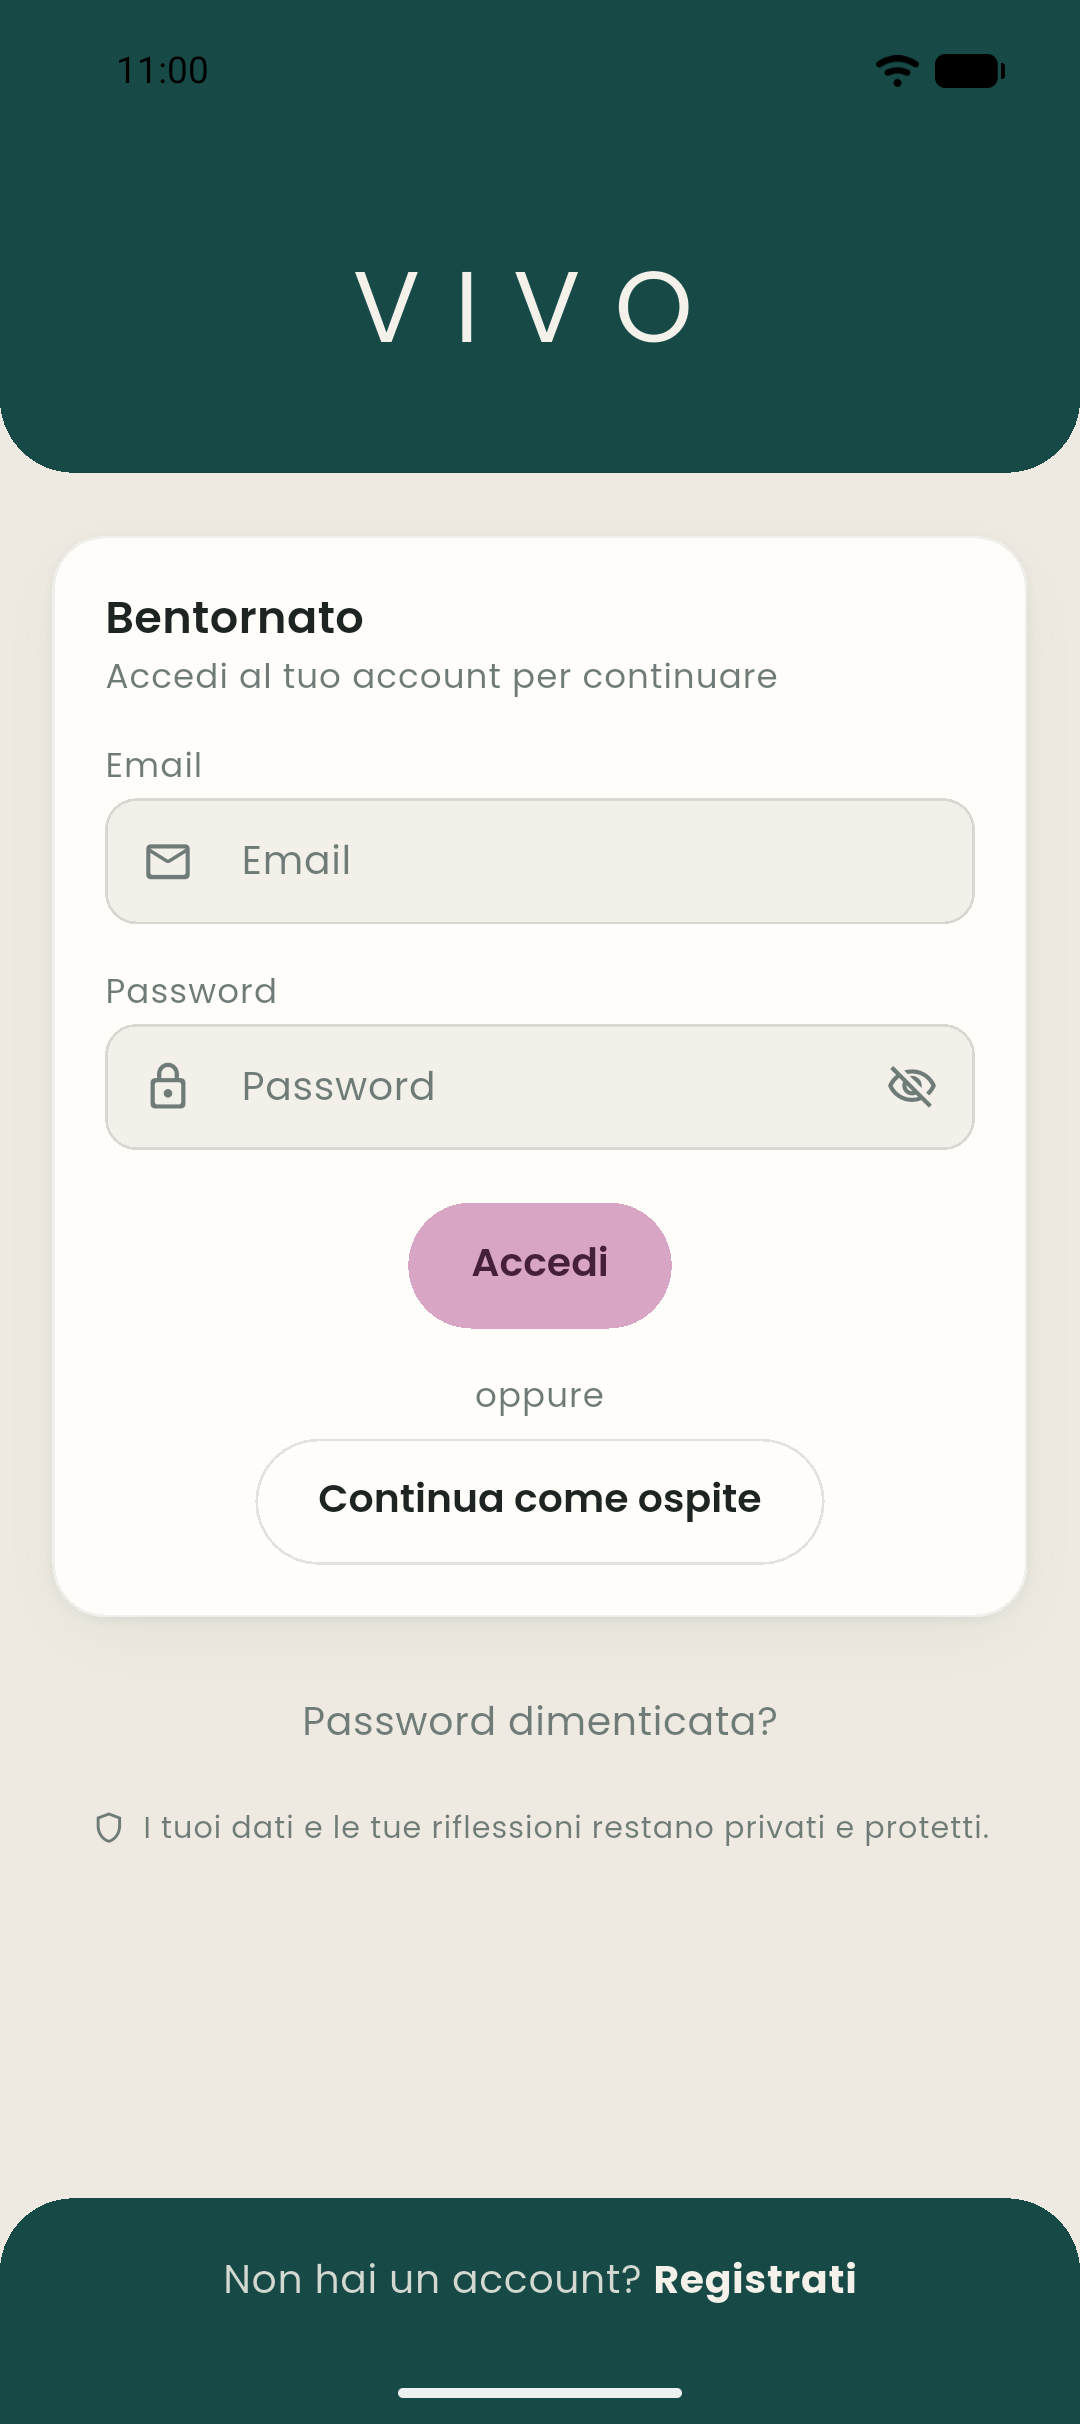
\includegraphics[height=8cm]{imgs/implementation/login.png}\hspace{1cm}
    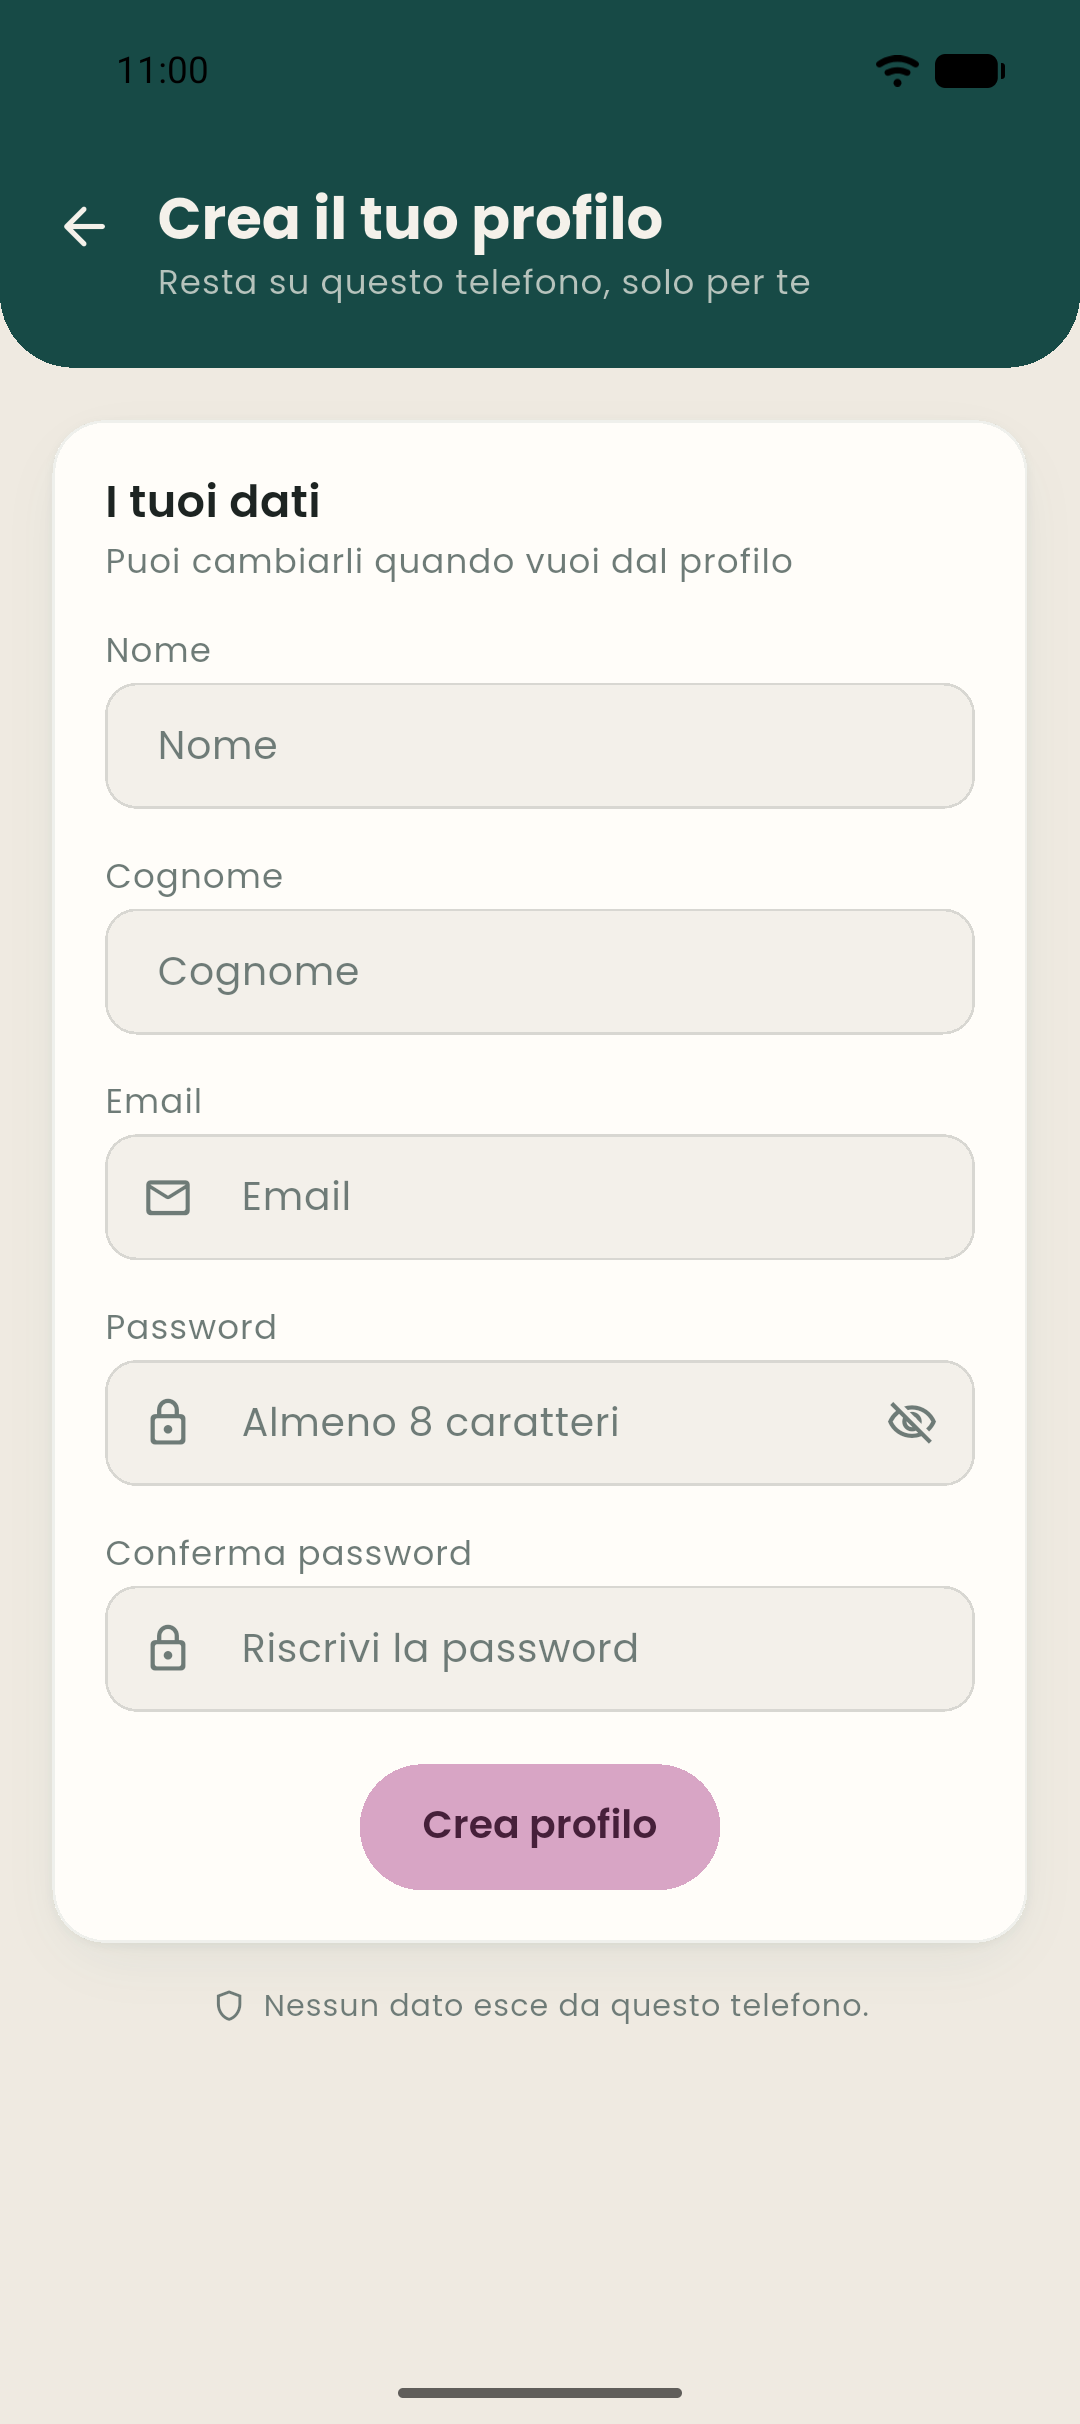
\includegraphics[height=8cm]{imgs/implementation/registrazione.png}
    \caption{Accesso e creazione del profilo nell'applicazione realizzata}
    \label{fig:impl-accesso}
\end{figure}

La schermata principale saluta l'utente per nome e riporta la data per esteso.
Il pulsante di aiuto è collocato a cavallo fra l'intestazione e il corpo, in una posizione che lo rende il primo elemento raggiunto dallo sguardo senza per questo occupare l'intera schermata.
Sotto di esso trovano posto la registrazione dell'umore quotidiano, le due attività avviabili in autonomia e la card dei progressi, che confronta il numero di richieste della settimana corrente con quello della settimana precedente e ne dichiara la variazione percentuale (\textbf{REQ-06}, \textbf{REQ-08}, \textbf{REQ-09}).

\begin{figure}[htbp]
    \centering
    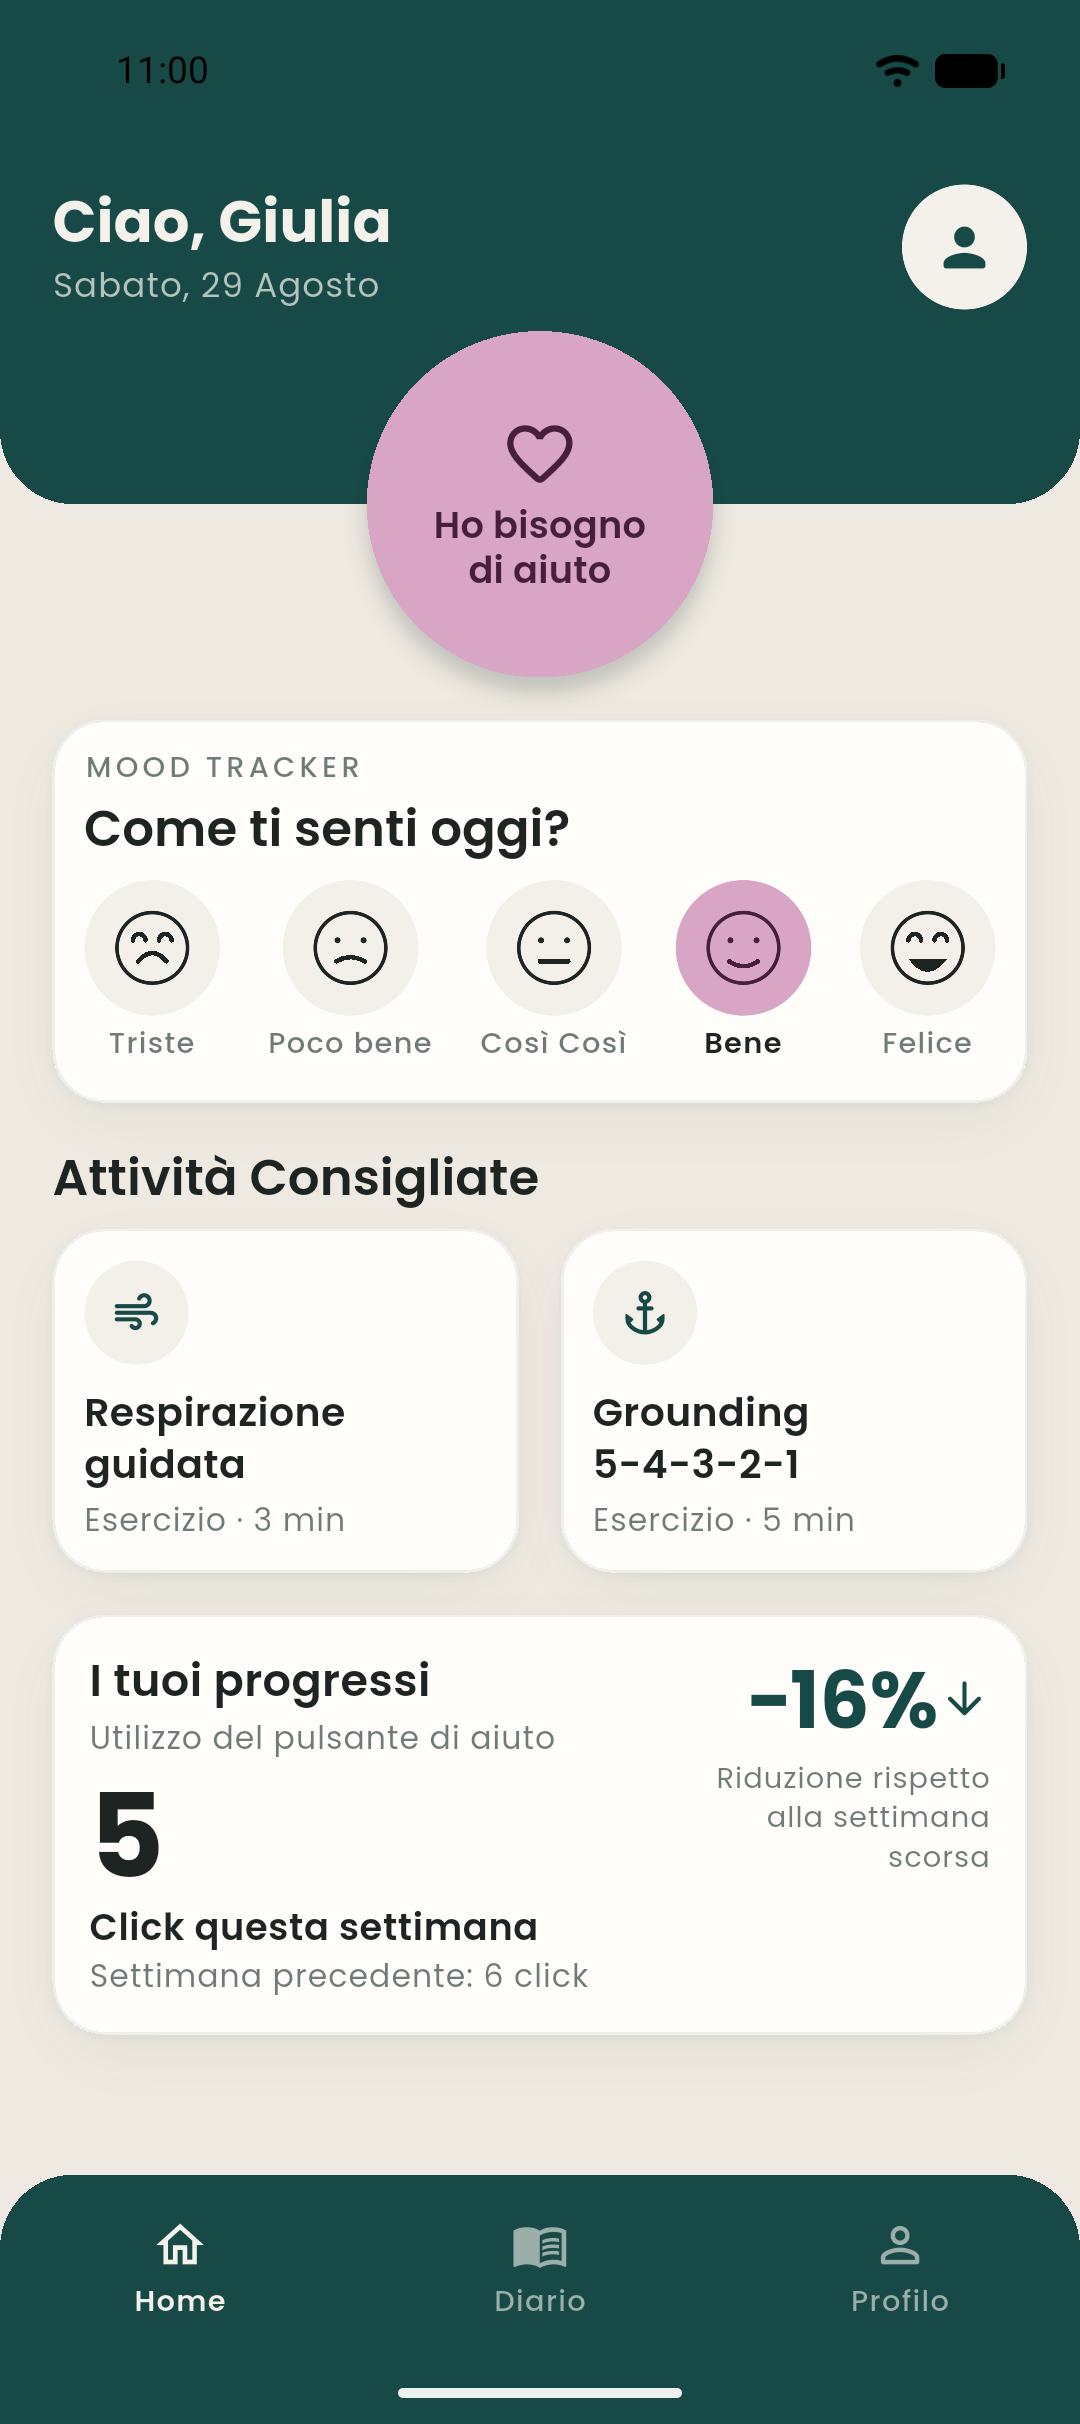
\includegraphics[height=8cm]{imgs/implementation/homepage.png}
    \caption{La schermata principale dell'applicazione realizzata}
    \label{fig:impl-homepage}
\end{figure}

Il percorso di aiuto si apre con la schermata di transizione, priva di comandi e di barre, che introduce la sessione con una frase e si esaurisce da sola dopo pochi secondi.
Le tre attività che seguono condividono la stessa cornice, composta dall'indicatore a tre passi in cima, dal titolo dell'esercizio con la relativa istruzione e dal comando di uscita esplicito.
La barra di navigazione inferiore, come stabilito dalla valutazione, non compare in nessuna di queste schermate (\textbf{REQ-03}).

\begin{figure}[htbp]
    \centering
    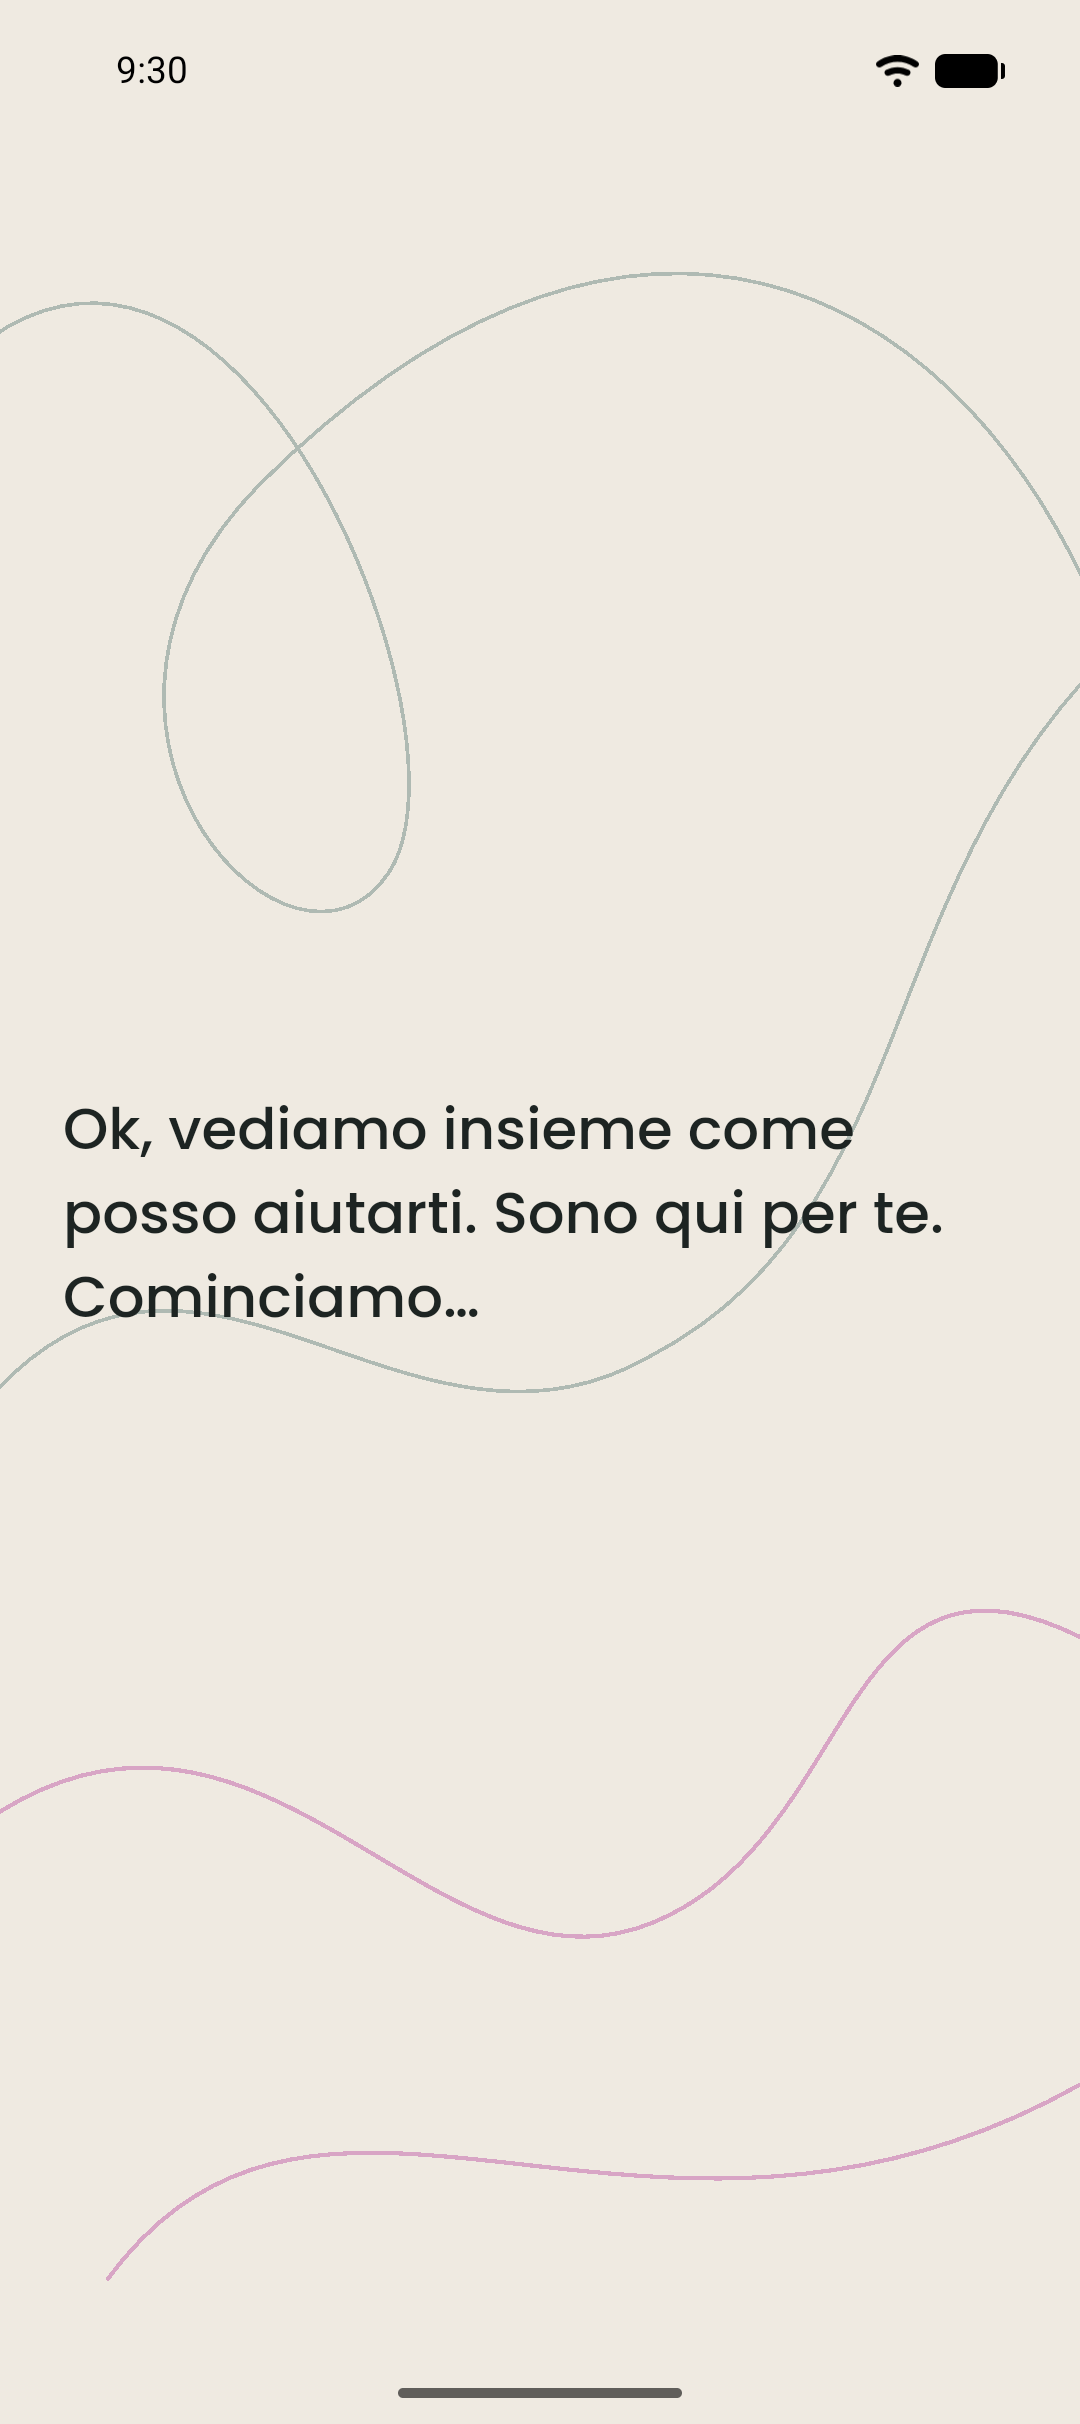
\includegraphics[height=7.5cm]{imgs/implementation/transizione.png}\hfill
    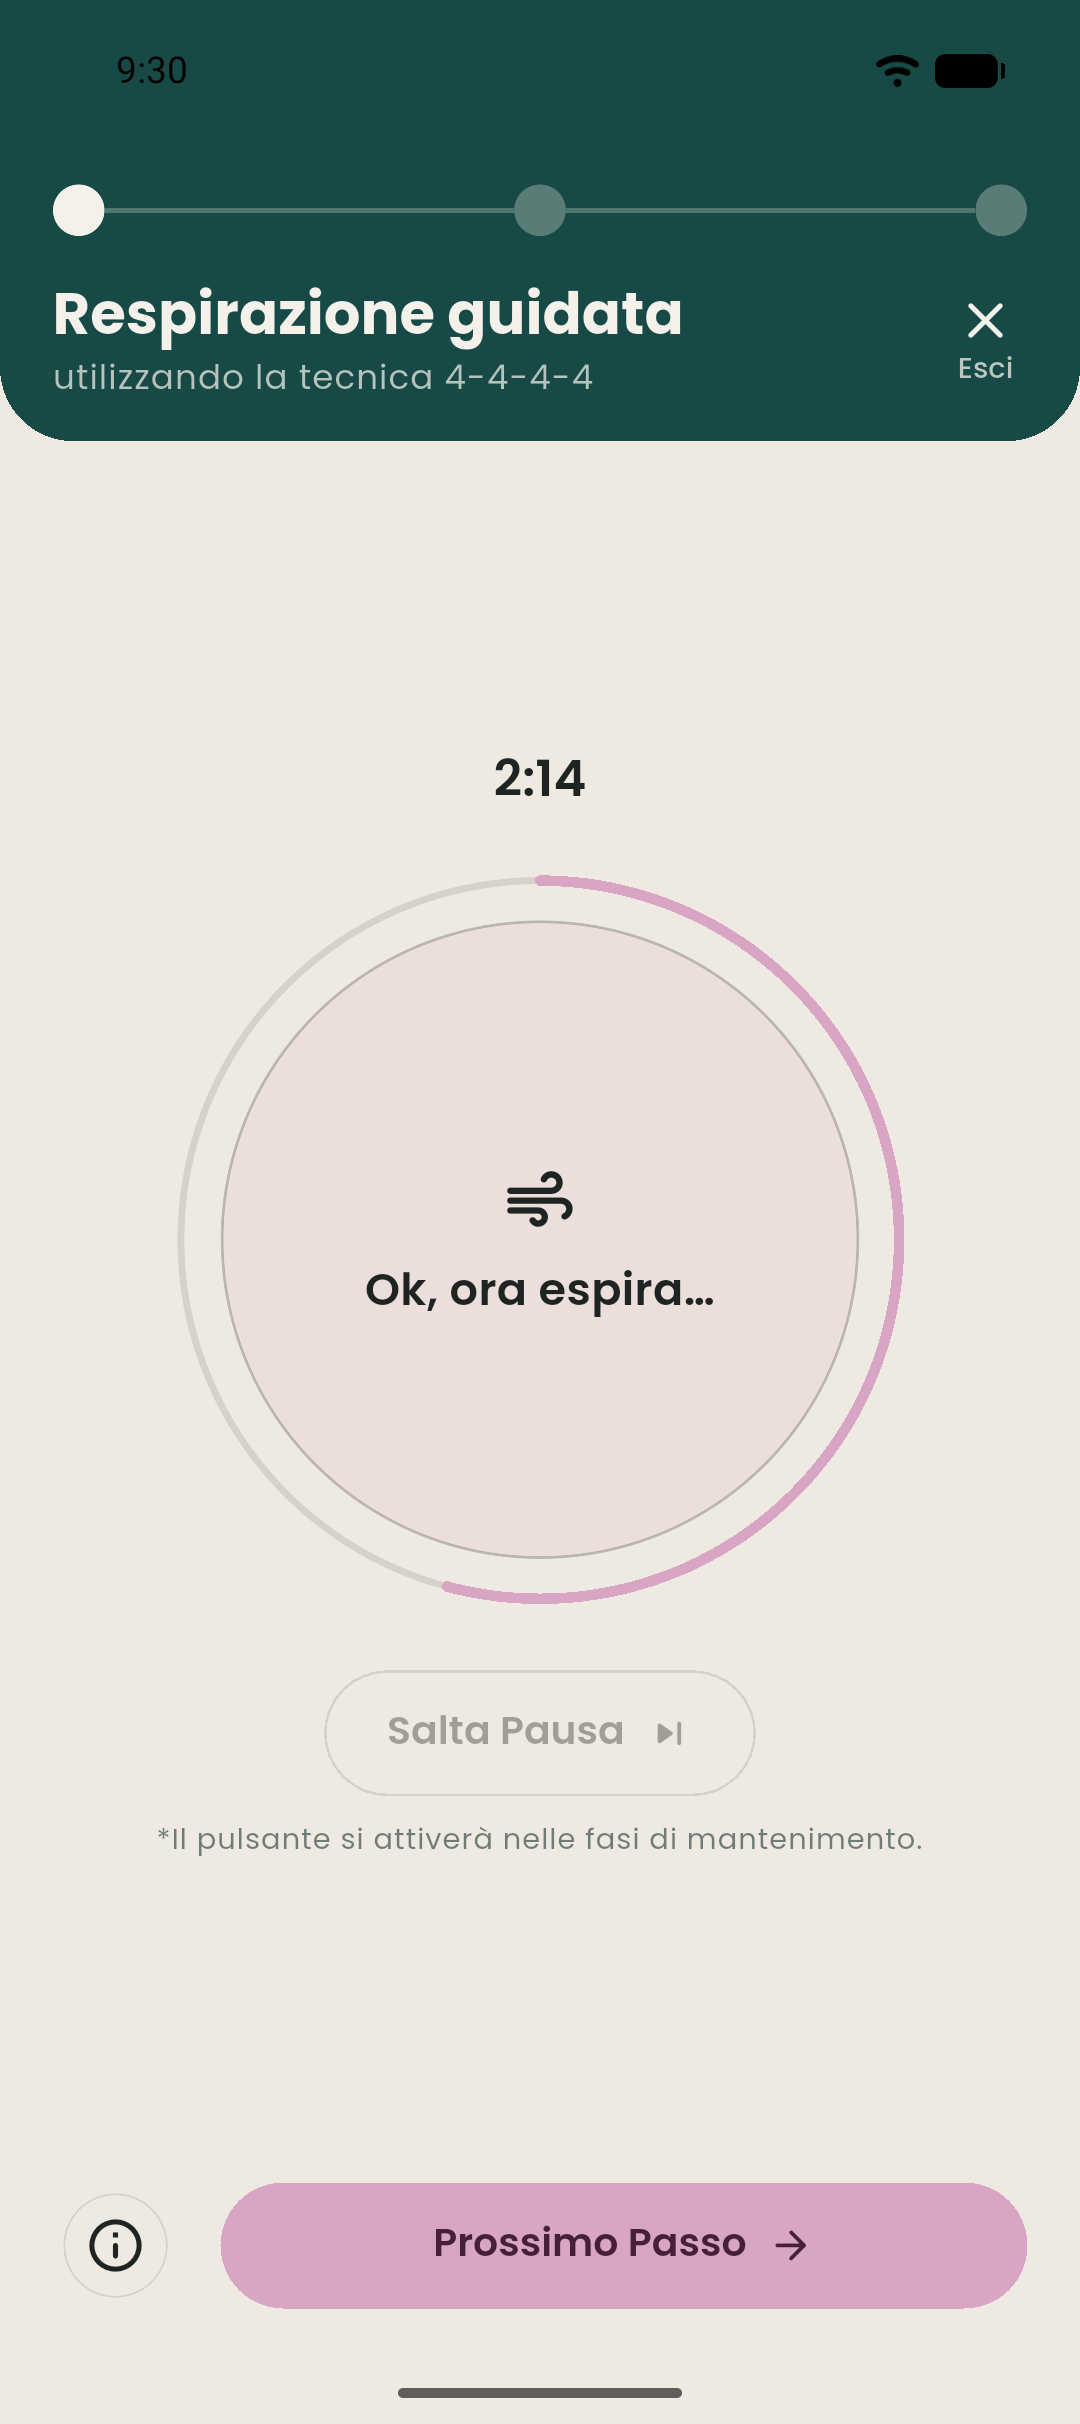
\includegraphics[height=7.5cm]{imgs/implementation/task-1.png}\hfill
    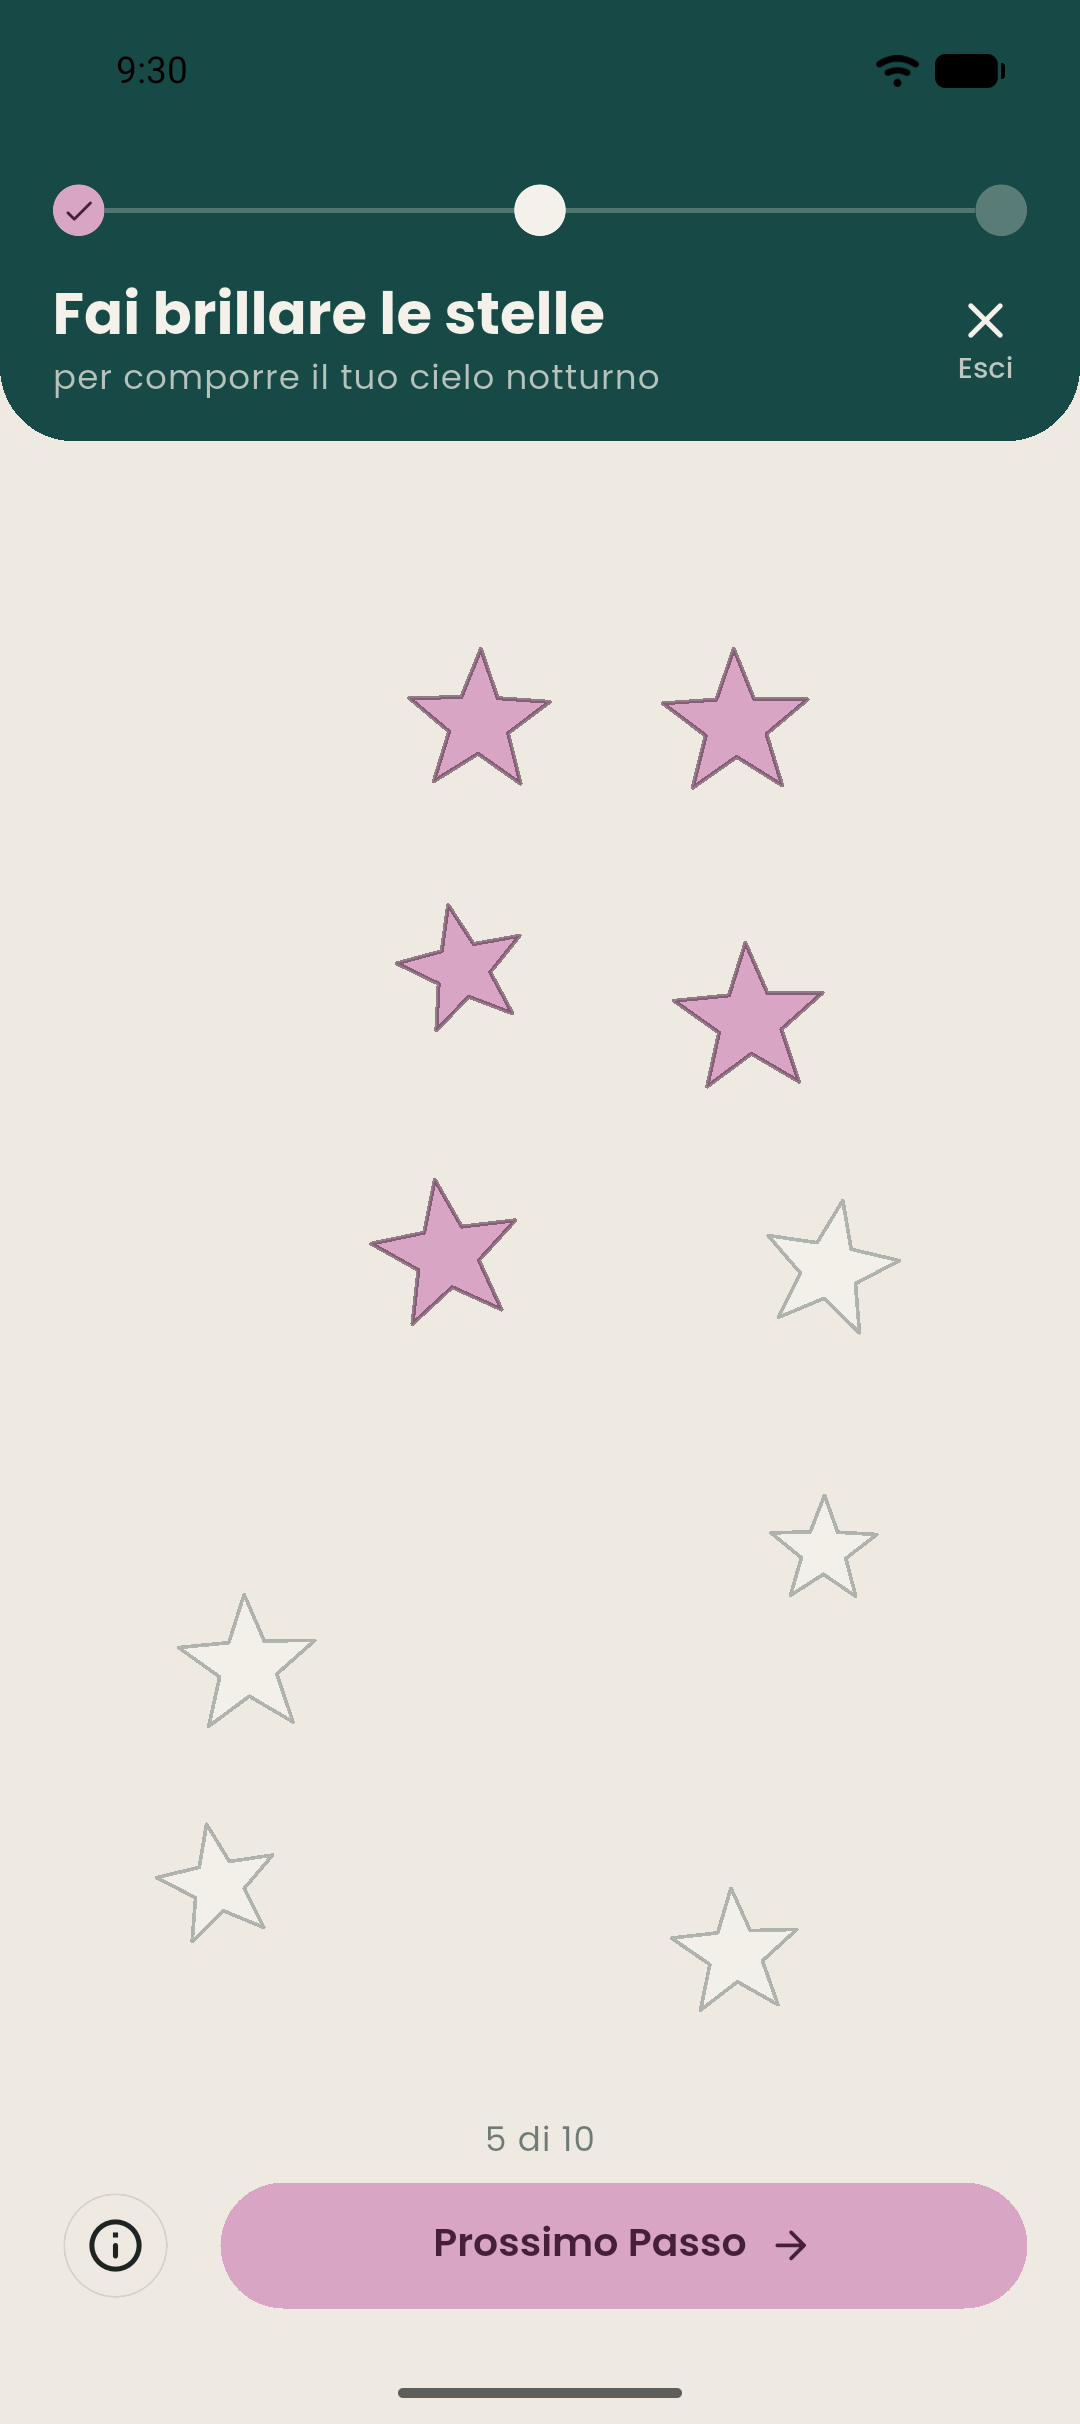
\includegraphics[height=7.5cm]{imgs/implementation/task-2.png}
    \caption{La transizione, la respirazione guidata e l'attività delle stelle}
    \label{fig:impl-flusso}
\end{figure}

La respirazione guidata mostra il tempo rimanente, un anello che avanza lungo il ciclo e un cerchio che si espande e si contrae accompagnando le fasi, con l'istruzione scritta al centro.
Il comando che salta le pause di mantenimento è stato reso esplicito dopo il test, e resta visibile ma inattivo fuori da quelle fasi, accompagnato da una riga che ne dichiara la condizione di attivazione, cosicché l'utente non lo cerchi invano né lo prema senza effetto.
L'attività delle stelle presenta un cielo di sagome da riempire con il tocco e un contatore che indica quante ne sono state accese, senza punteggi né tempi da rispettare.
Il grounding si sviluppa come una sequenza verticale in cui il passo corrente è pienamente leggibile mentre quelli successivi restano accennati, e si rivelano soltanto procedendo, per non mettere davanti agli occhi di chi è in difficoltà l'intero compito in una volta sola.

\begin{figure}[htbp]
    \centering
    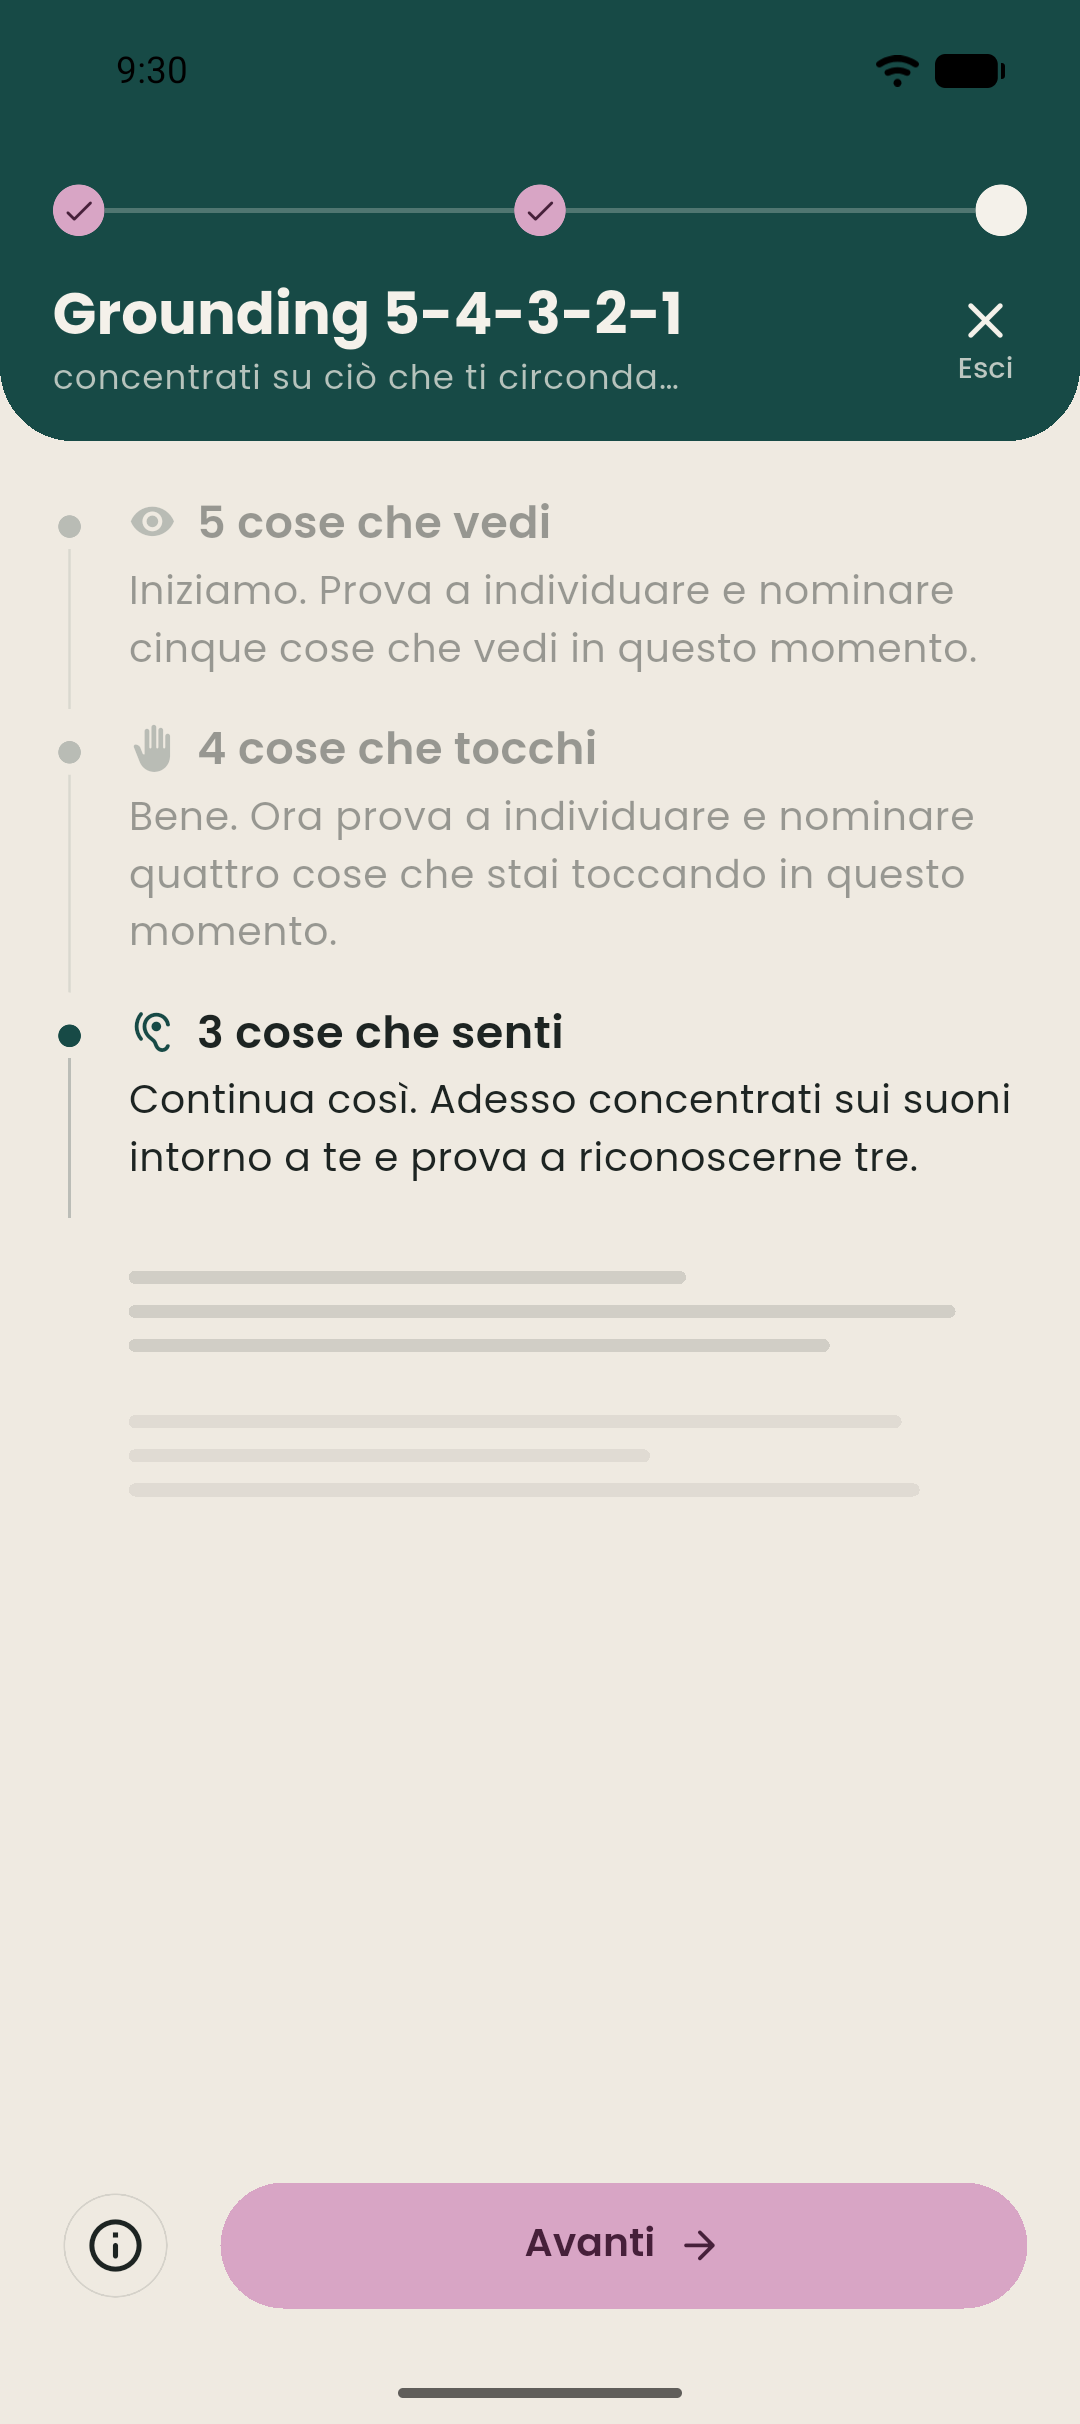
\includegraphics[height=8cm]{imgs/implementation/task-3.png}\hspace{1cm}
    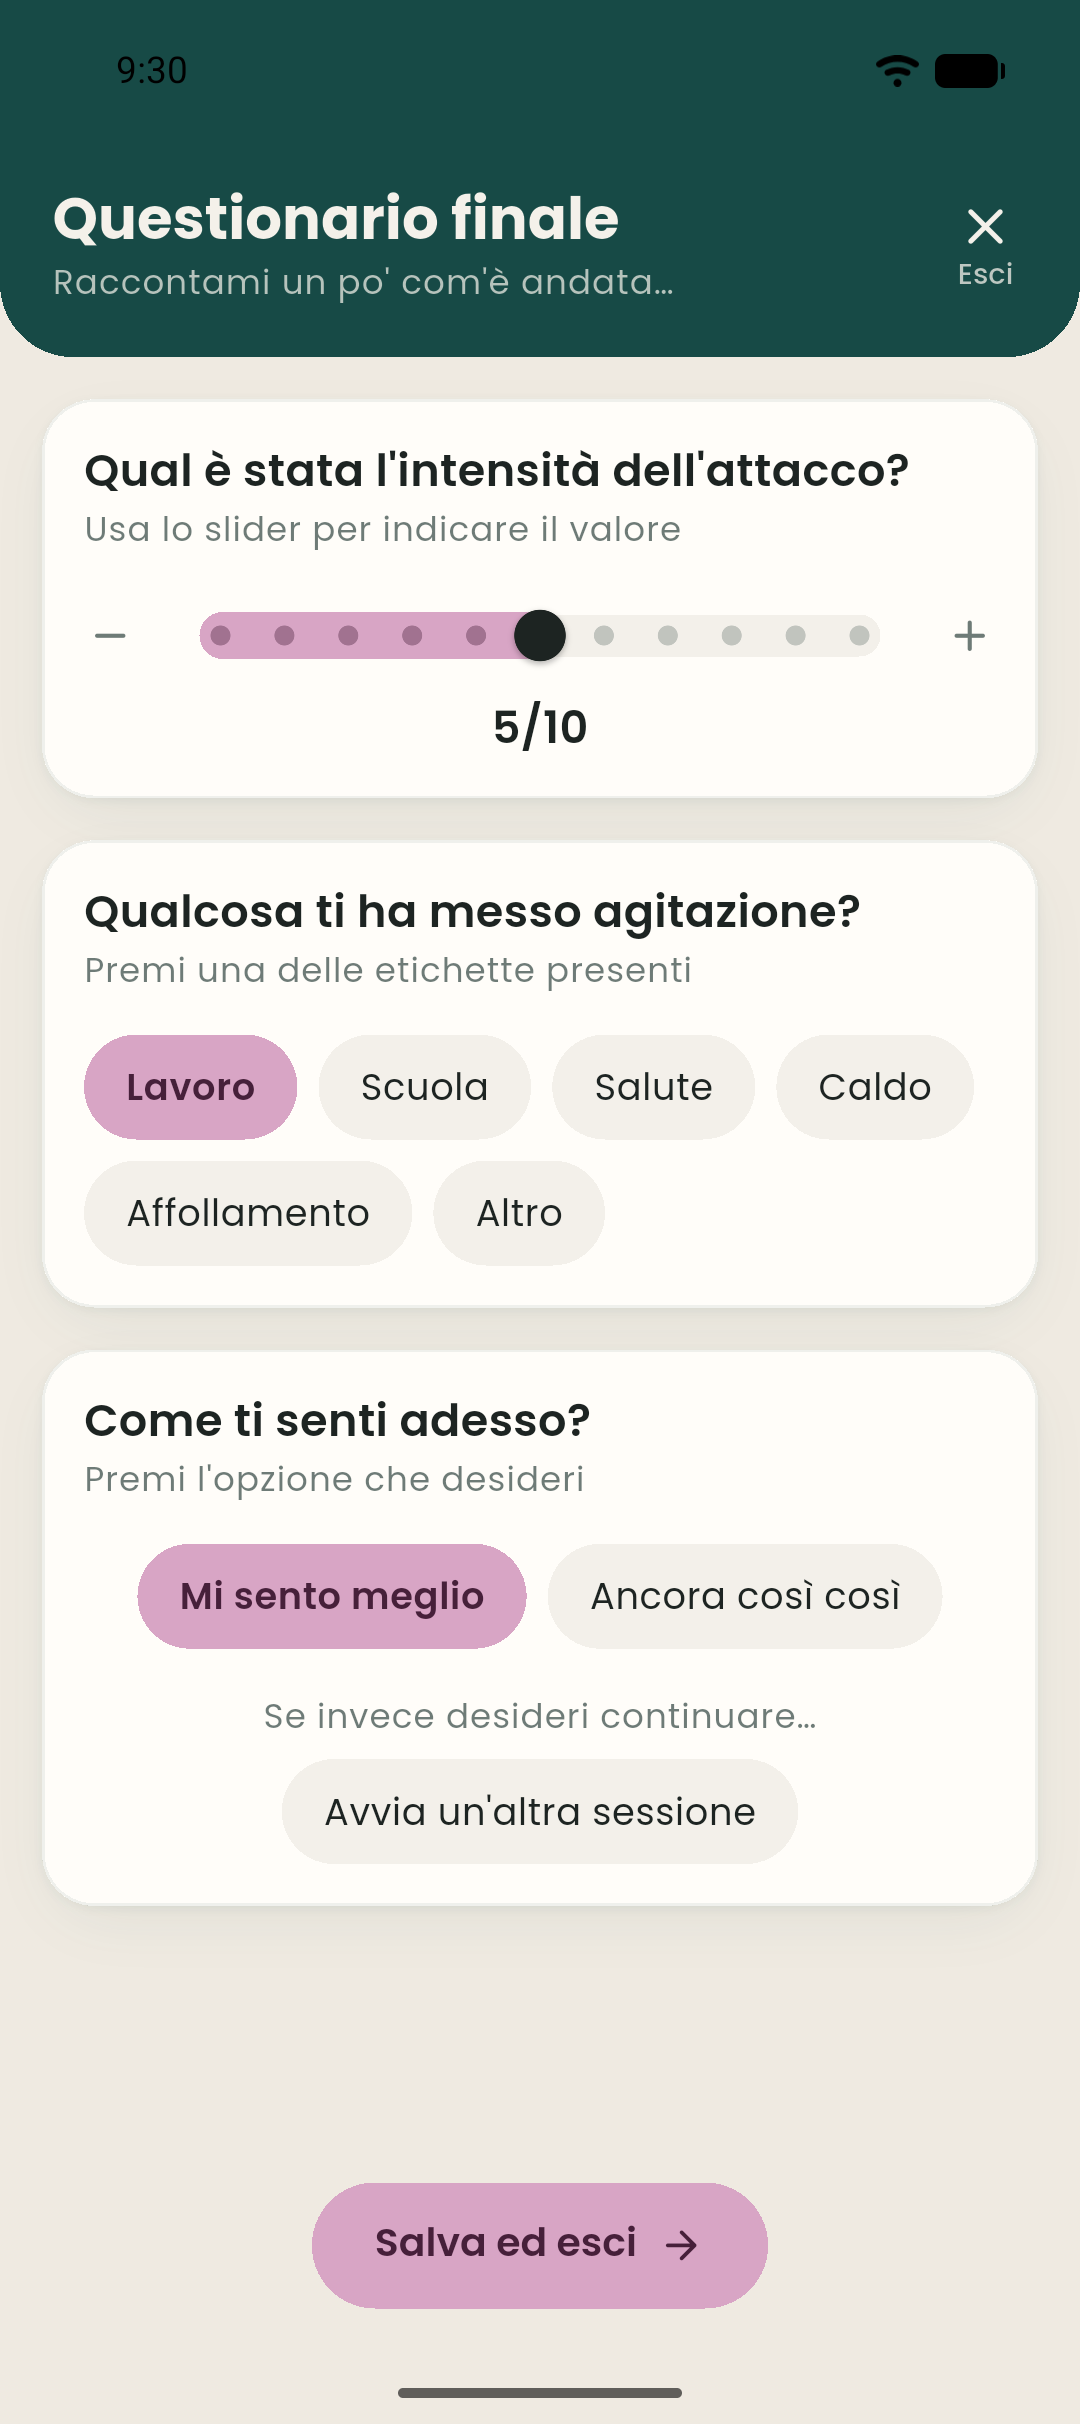
\includegraphics[height=8cm]{imgs/implementation/questionario.png}
    \caption{Il grounding 5-4-3-2-1 e il questionario di chiusura}
    \label{fig:impl-questionario}
\end{figure}

Il questionario conclusivo raccoglie in tre card l'intensità dichiarata su una scala da zero a dieci, il fattore scatenante scelto fra etichette già pronte fra cui compare quella generica, e lo stato dell'utente al termine della sessione.
A quest'ultima domanda è affiancata la possibilità di avviare immediatamente un altro percorso, per il caso in cui il primo non sia bastato.
L'intestazione conserva il comando di uscita, e il pulsante conclusivo dichiara nel proprio testo che il salvataggio coincide con l'uscita (\textbf{REQ-06}).

Il diario si apre su un calendario mensile in cui i giorni che contengono registrazioni sono contrassegnati da un punto, così che lo storico si attraversi senza scorrere elenchi (\textbf{REQ-07}).
Sotto il calendario, la giornata selezionata è riassunta dall'umore registrato e dalla card delle richieste di aiuto, che riporta per ciascun episodio il numero progressivo, l'orario e l'intensità.
Il riquadro di dettaglio, adottato nella forma scelta dagli utenti, raccoglie tutti gli episodi della giornata in un unico blocco e affianca a ogni valore una barra proporzionale e il fattore scatenante.
La riflessione della giornata occupa la parte inferiore della schermata e si apre in un riquadro dedicato alla sola scrittura, modificabile anche in un momento successivo (\textbf{REQ-10}).

\begin{figure}[htbp]
    \centering
    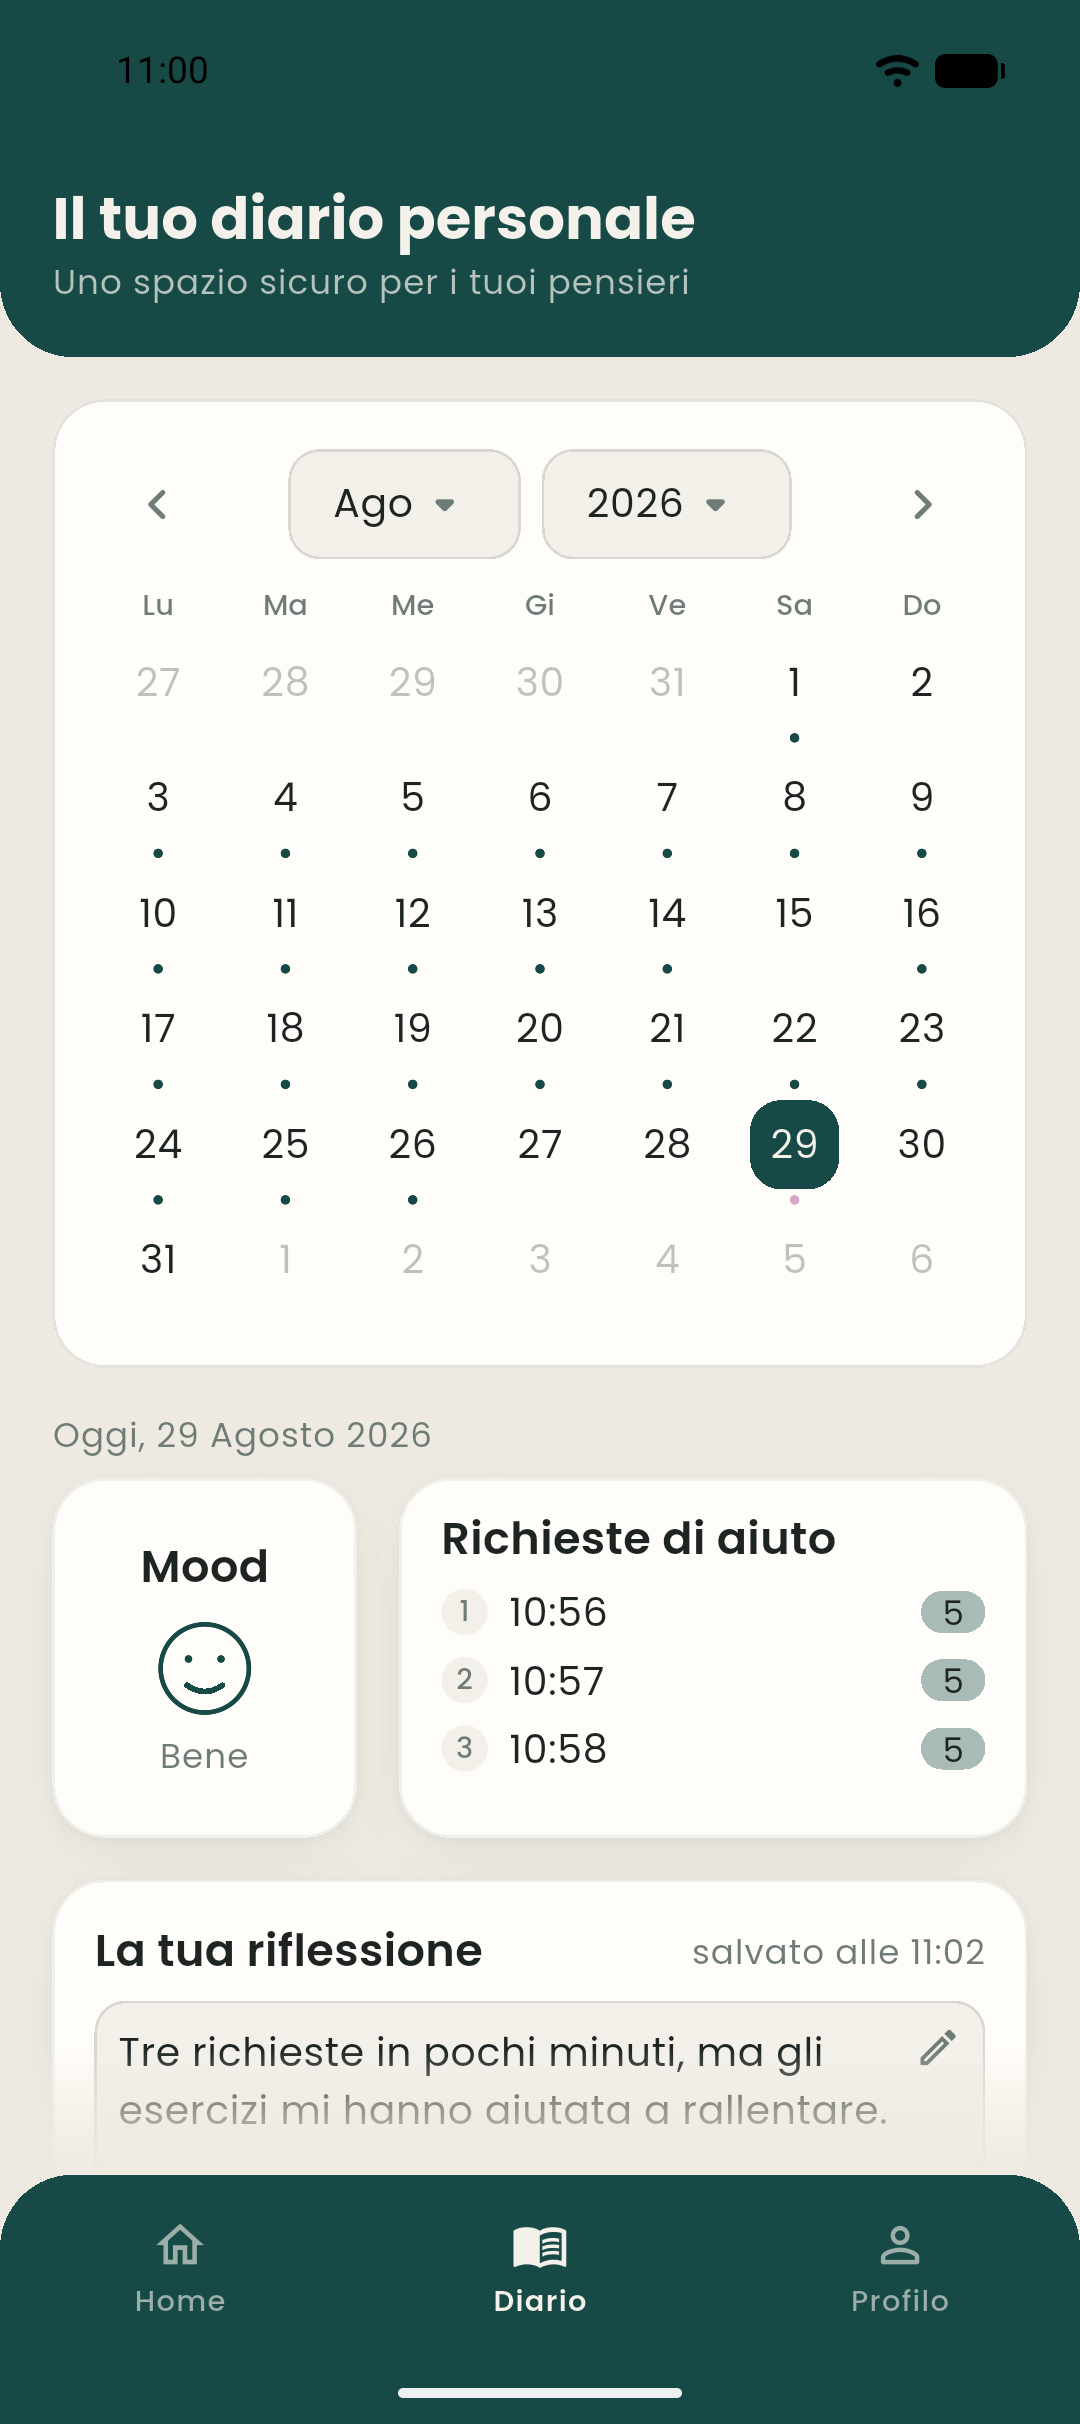
\includegraphics[height=7.5cm]{imgs/implementation/diario.png}\hfill
    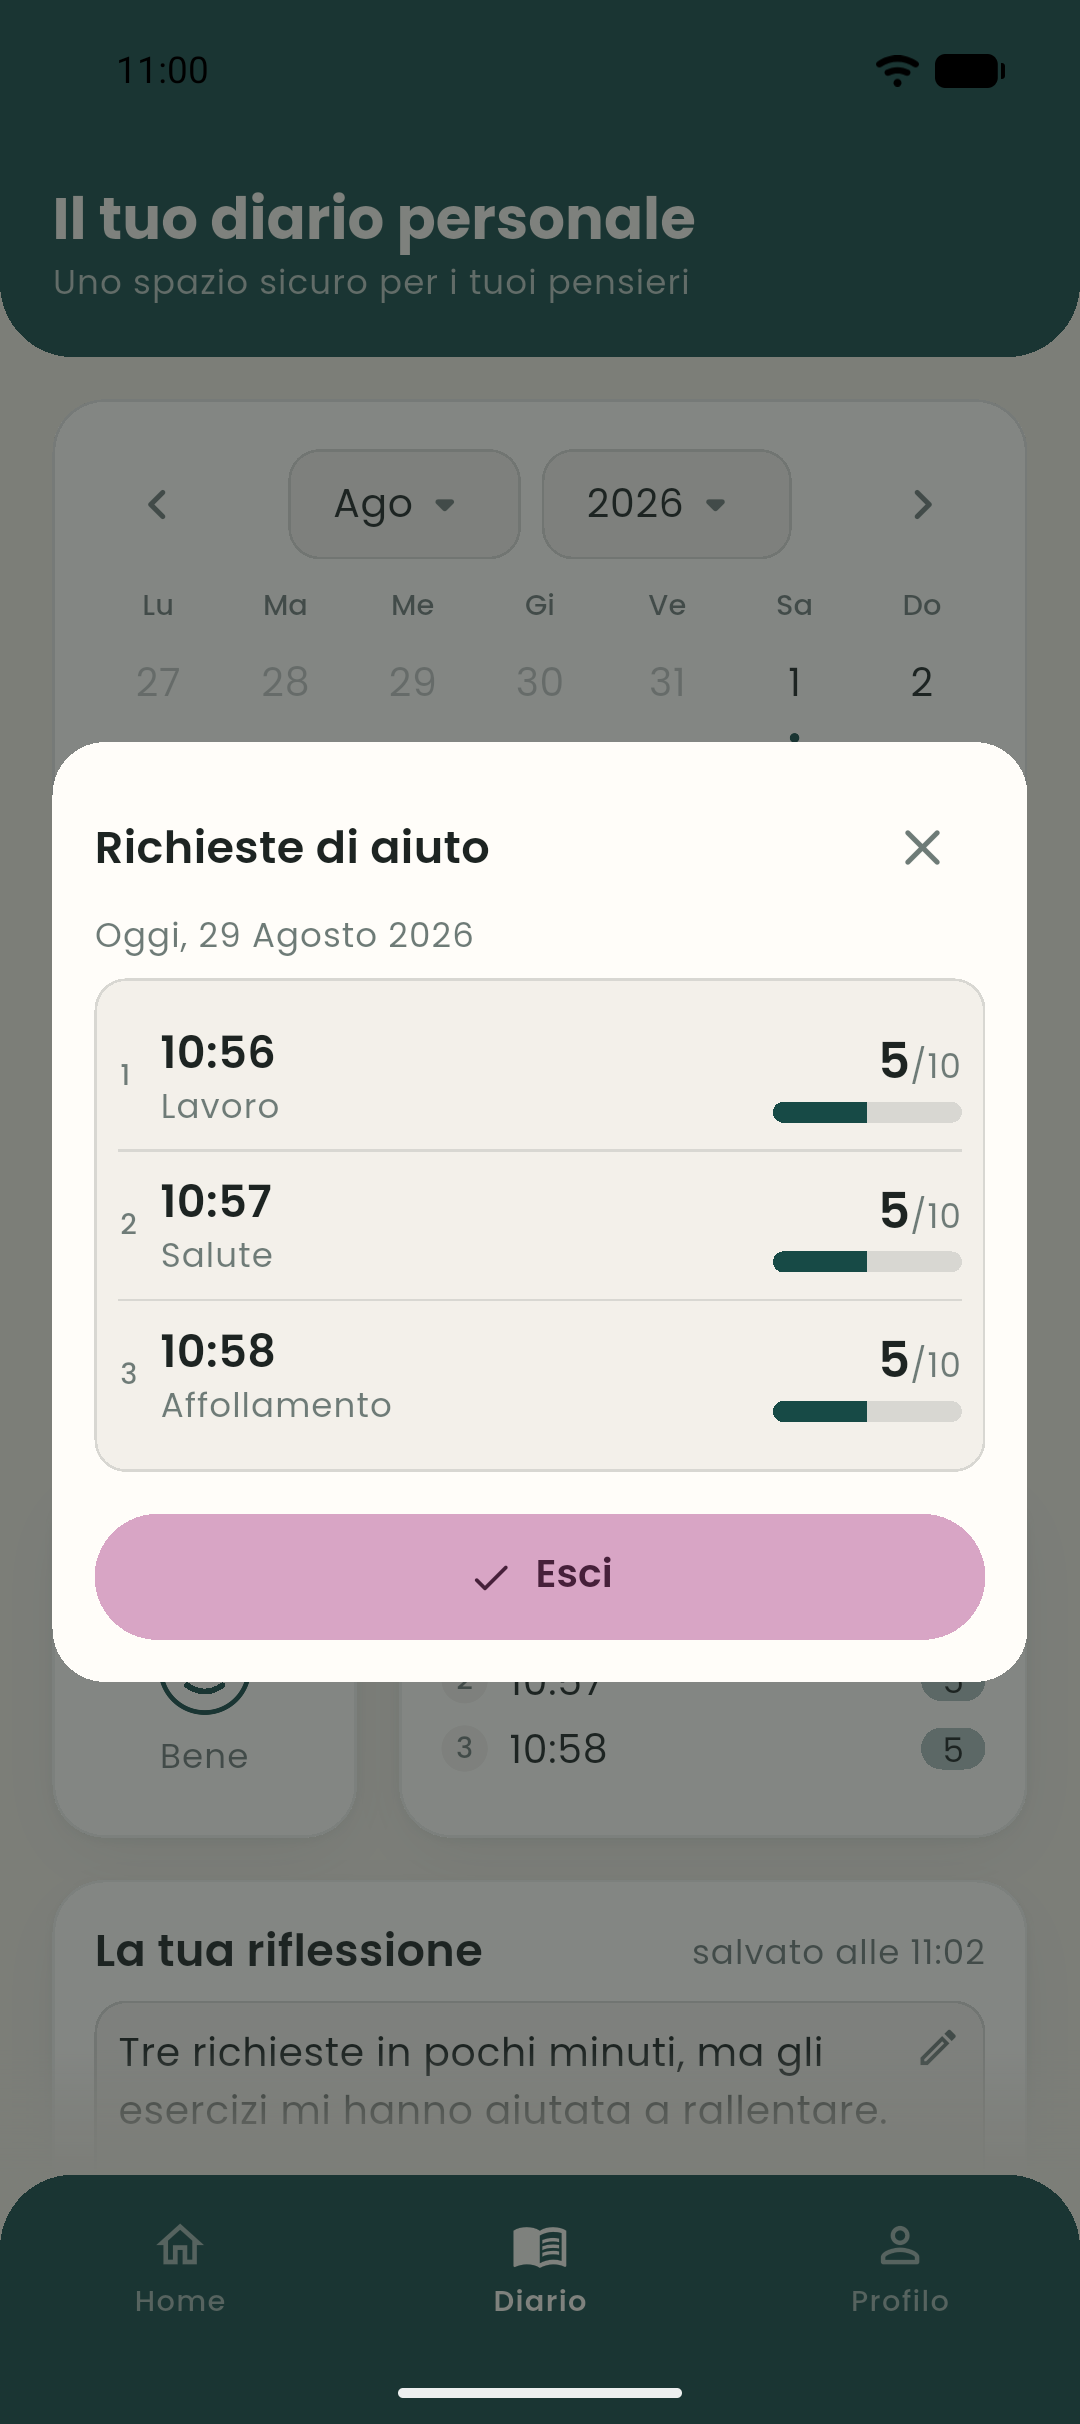
\includegraphics[height=7.5cm]{imgs/implementation/popup-richieste-aiuto.png}\hfill
    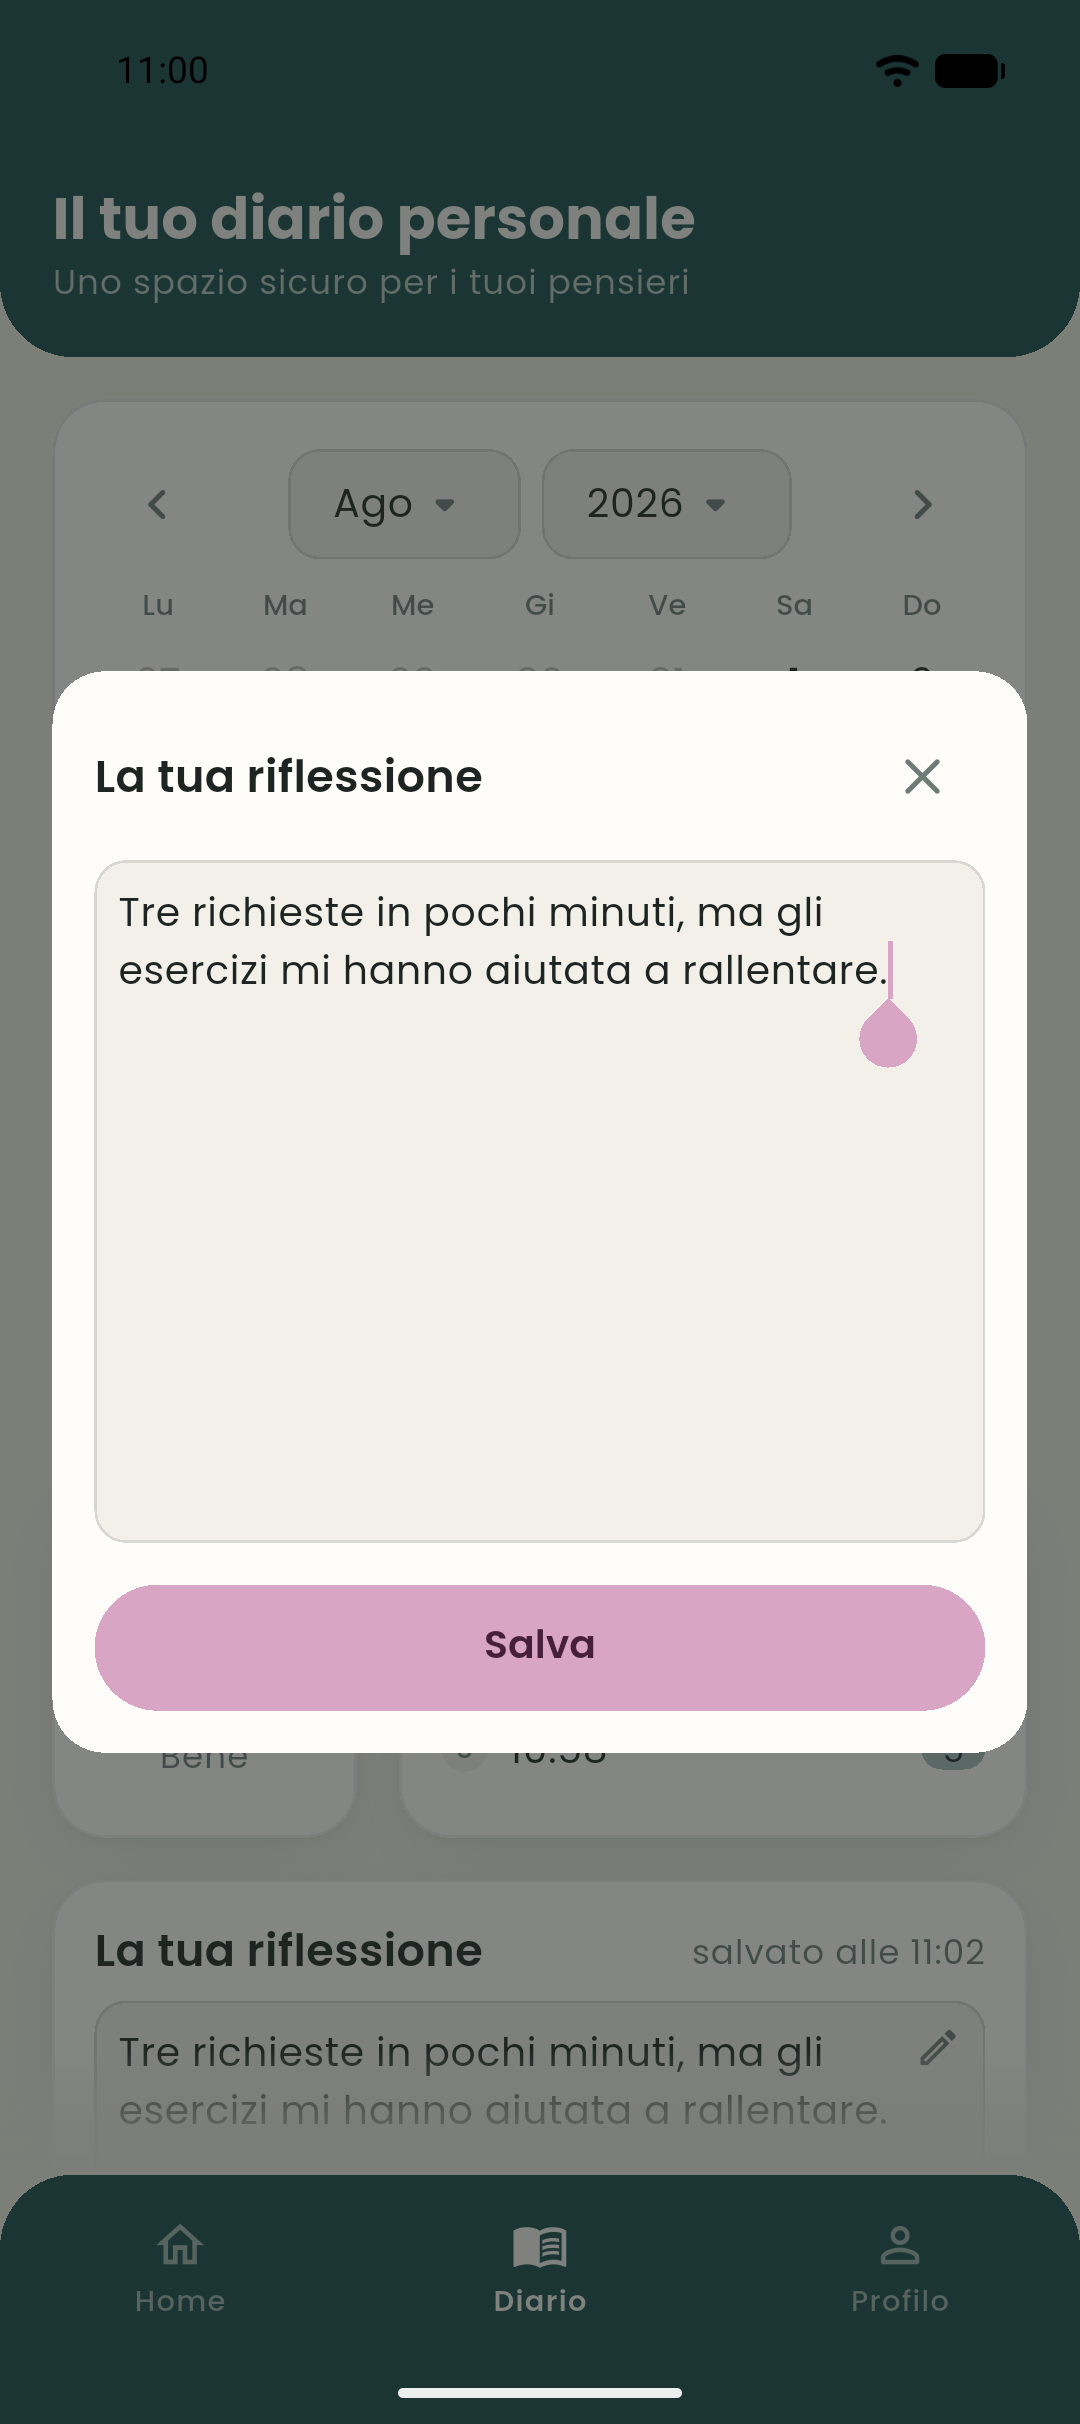
\includegraphics[height=7.5cm]{imgs/implementation/popup-riflessione.png}
    \caption{Il diario, il dettaglio delle richieste di aiuto e la riflessione personale}
    \label{fig:impl-diario}
\end{figure}

Il profilo raccoglie nella prima card i dati personali, con l'immagine scelta dalla galleria o dalla fotocamera, e nella seconda le impostazioni, dove l'interruttore del promemoria è affiancato dal cambio della password e dalla disconnessione (\textbf{REQ-11}).
L'eliminazione dell'account resta isolata in fondo alla schermata, con un trattamento visivo che ne abbassa deliberatamente il peso rispetto alle azioni ordinarie, e la cancellazione rimuove dal dispositivo l'intero archivio dell'utente (\textbf{REQ-05}).

\begin{figure}[htbp]
    \centering
    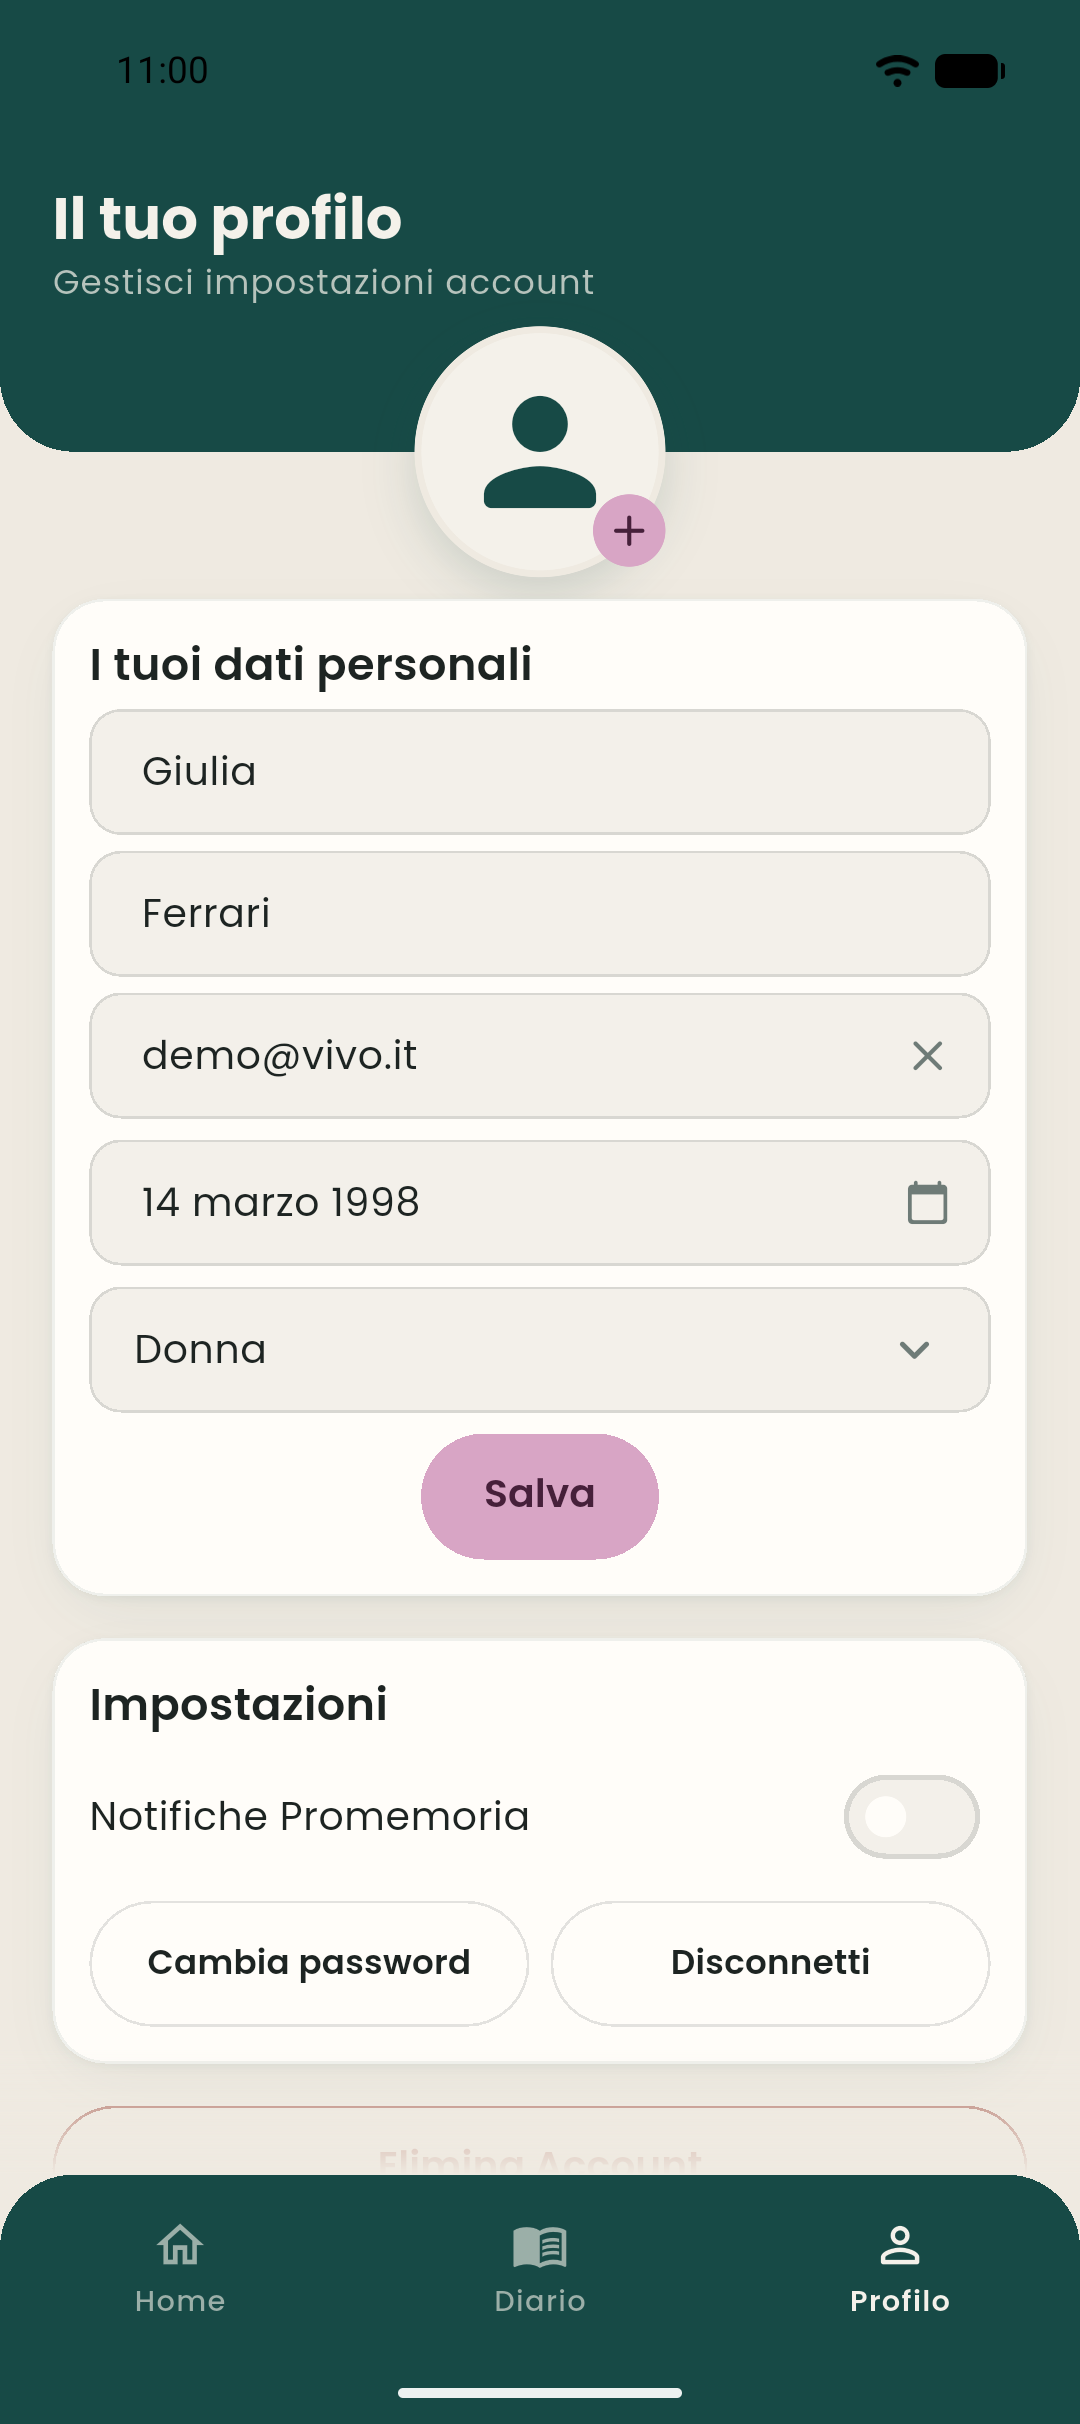
\includegraphics[height=8cm]{imgs/implementation/profilo.png}
    \caption{Il profilo dell'applicazione realizzata}
    \label{fig:impl-profilo}
\end{figure}

\section{Differenze rispetto alla progettazione}
\label{sec:differenze}

Lo sviluppo ha confermato l'architettura definita nei wireframe, ma alcune scelte sono state riviste nel passaggio all'applicazione funzionante.
Il confronto è stato condotto schermata per schermata, ridisegnando ciascuna interfaccia dal codice sulle misure del wireframe corrispondente e mettendo le due immagini a fianco.
Di seguito sono riportate le differenze che cambiano il modo in cui l'applicazione si usa, mentre gli scarti di sola resa tipografica, come il corpo di un testo o il centraggio verticale di un blocco, non compaiono nell'elenco perché non incidono su ciò che l'utente può fare.

\textbf{L'intensità nella card del diario.}
Il wireframe scelto dagli utenti affidava l'intensità a una pastiglia riempita per una lunghezza proporzionale al valore.
Nell'applicazione la pastiglia resta, ma è la sua tinta a farsi più carica quanto più l'intensità è alta, mentre il riempimento proporzionale è stato spostato nel riquadro di dettaglio, dove ogni episodio dispone della larghezza intera e la barra si legge accanto al fattore scatenante.
Il risultato cercato dal test non cambia, poiché scorrendo l'elenco la giornata si legge prima dei numeri, ma la forma dell'indicatore non è quella valutata e va dichiarata (\textbf{REQ-07}).

\textbf{Il contatore delle stelle.}
Né lo sketch né il wireframe indicavano quante stelle fossero già state accese, e il cielo si presentava come un compito senza misura.
L'applicazione riporta il conteggio sotto le sagome, nella forma \enquote{5 di 10}, che restituisce il progresso senza trasformarlo in una condizione da soddisfare, dal momento che il passaggio all'attività successiva resta disponibile in qualsiasi momento (\textbf{REQ-03}).

\textbf{Il comando della riflessione.}
Lo sketch dichiarava insieme il salvataggio e l'uscita con la formula \enquote{Salva ed esci}.
Nel wireframe e nell'applicazione il comando si riduce alla sola parola \enquote{Salva}, poiché il riquadro si chiude riportando al diario, che resta visibile dietro di esso per tutto il tempo della scrittura.

\textbf{Il velo dei riquadri del diario copre anche la barra di navigazione.}
Nel wireframe la barra in fondo resta illuminata mentre il riquadro della riflessione è aperto, e quindi raggiungibile durante la scrittura.
Nell'applicazione il velo la copre insieme al resto della schermata, e un tocco fuori dal riquadro lo chiude anziché cambiare scheda.
Una barra attiva accanto a un testo non ancora salvato è la stessa via d'uscita involontaria che la valutazione aveva rilevato nel percorso di aiuto, e la soluzione adottata è la medesima (\textbf{REQ-03}).

\textbf{Il saluto della schermata principale è fisso.}
Il wireframe mostra un saluto legato all'ora del giorno, del tipo \enquote{Buongiorno}, mentre l'applicazione scrive sempre \enquote{Ciao} seguito dal nome.
Con un nome reale accanto, la formula contestuale mandava il saluto su due righe dell'intestazione, e la riga in più costava alla schermata più di quanto il saluto aggiungesse.

\textbf{Il calendario del diario comincia di lunedì.}
Il wireframe disegnava la settimana a partire da domenica.
La settimana che inizia di lunedì è la convenzione in uso in Italia ed è la stessa adottata dal calcolo dell'andamento settimanale (\textbf{REQ-09}), cosicché il conteggio dei progressi e le colonne del calendario si riferiscano allo stesso periodo.

\textbf{La dimensione del carattere.}
Quest'ultima voce non è uno scostamento dal disegno, che sul punto non diceva nulla, ma una scelta dello sviluppo che va dichiarata.
L'applicazione impiega la propria scala tipografica e ignora la dimensione del carattere impostata nel telefono.
La scelta preserva i layout valutati con gli utenti, che con i corpi di testo più grandi manderebbero a capo i titoli delle card, ma costituisce anche un limite di accessibilità dichiarato, ripreso fra gli sviluppi futuri.

Una parola infine sul modo in cui il confronto è stato condotto.
Non tutte le differenze rilevate sono state accettate a tavolino: quella relativa allo stacco fra il pannello del logo e la card nella schermata di accesso, che nel disegno è più ampio di quanto l'applicazione mostri, è stata corretta davvero, ricostruendo il pacchetto e installandolo per osservare le due versioni sul dispositivo.
A confronto diretto, e persino ingrandendo le immagini, la modifica non risultava distinguibile, e per questo è stata annullata.
Una differenza che nessuno percepisce non giustifica un intervento sulla prima schermata dell'applicazione.
